\documentclass[
aspectratio=169,
]{beamer}

\usepackage[english]{babel}
\usepackage[utf8]{inputenc}
\usepackage[T1]{fontenc}
\usepackage{booktabs}
\usepackage{url}
\usepackage{siunitx}
\usepackage{listings}
\usetheme[
  workplace=fi,
]{MU}

\definecolor{background}{HTML}{F5DD9D}
\definecolor{symbolColorTop}{HTML}{FFECB3}
\definecolor{symbolColorBox}{HTML}{FFF9E5}
\definecolor{gray}{rgb}{0.25,0.25,0.25}
\definecolor{darkblue}{rgb}{0.0,0.0,0.6}
\definecolor{cyan}{rgb}{0.0,0.6,0.6}
\definecolor{lightblue}{rgb}{0.9,0.95,1.0}
\definecolor{darkgreen}{rgb}{0.0,0.6,0.0}
\definecolor{brown}{HTML}{A52A2A}
\definecolor{darkmagenta}{HTML}{8B008B}

\lstset{
	basicstyle      = \ttfamily,%
	identifierstyle = \color{black},%
	keywordstyle    = \color{blue},%
	keywordstyle    = {[2]\color{cyan}},%
	keywordstyle    = {[3]\color{olive}},%
	stringstyle     = \color{teal},%
	commentstyle    = \itshape\color{magenta}}

\newcommand\Cpp{
	\lstset{
		basicstyle=\ttfamily,
		columns=fullflexible,
		showstringspaces=false,
		tabsize=4,
		numbers=left,
		xleftmargin=2em,
		backgroundcolor = \color{lightblue},
		language=C++,
		identifierstyle=\color{brown},
		keywordstyle=\color{blue},
		stringstyle=\color{red},
		commentstyle=\color{darkgreen},
		morecomment=[l][\color{darkmagenta}]{\#}
	}
}

\begin{document}

\title[FreeRTOS]{FreeRTOS}
\subtitle[Real-time operating system for microcontrollers]{Real-time operating system for microcontrollers}
\author[B.\,Said]{Bed\v{r}ich Said \\ 409874@mail.muni.cz}
\institute[FI MU]{Faculty of Informatics, Masaryk University}
\date{\today}
\subject{Presentation Subject}
\keywords{the, presentation, keywords}

\begin{frame}[plain]
\maketitle
\end{frame}

\section[FreeRTOS and used hardware]{FreeRTOS and used hardware}

\begin{frame}
	\begin{block}{What you can find in this presentation}
		\begin{itemize}
			\item FreeRTOS implementation in ESP32
			\item The basics of FreeRTOS in examples
			\item Concurrent data structures included in FreeRTOS
		\end{itemize}
	\end{block}
	\begin{exampleblock}{What is not included}
		\begin{itemize}
			\item No deep theory and details about RTOS
			\item No other RTOS than FreeRTOS
			\item Nothing about how to compile and run FreeRTOS under your platform
		\end{itemize}
	\end{exampleblock}
\end{frame}

\begin{frame}{Overview}
	\tableofcontents[currentsection]
\end{frame}

\begin{frame}{FreeRTOS webpage}
	\begin{center}
		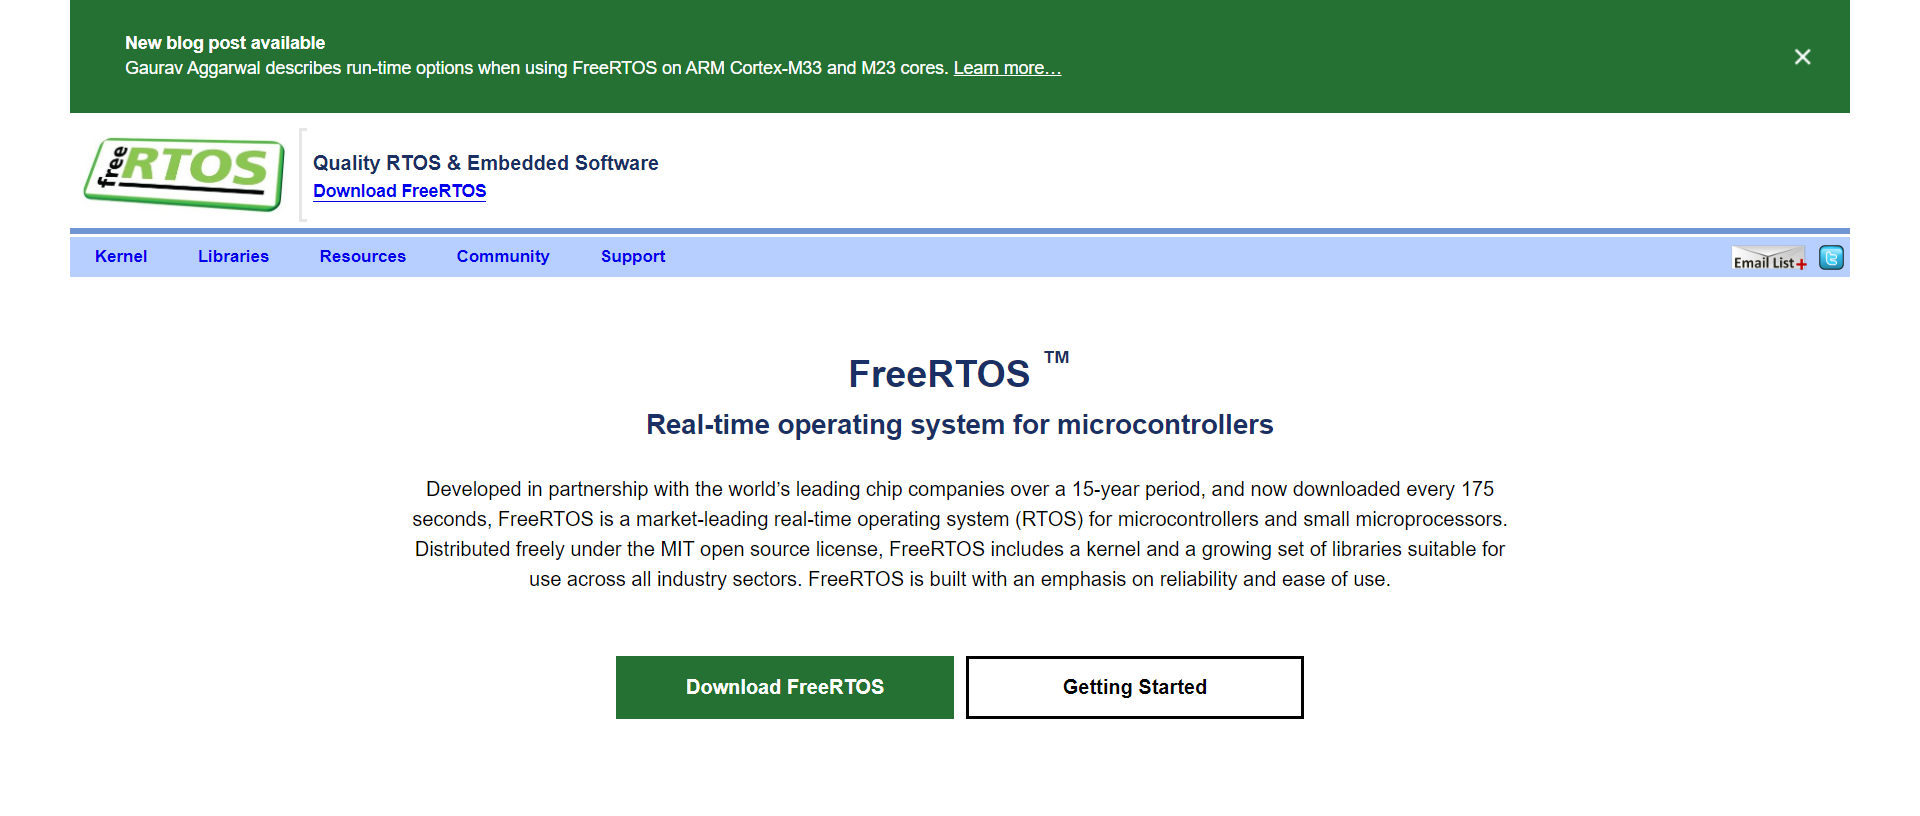
\includegraphics[width=\textwidth]{img/screencapture-freertos-org.png}\\
		\url{https://www.freertos.org/}
	\end{center}
\end{frame}

\begin{frame}{We will work with ESP32 dual core processor}
	\begin{center}
		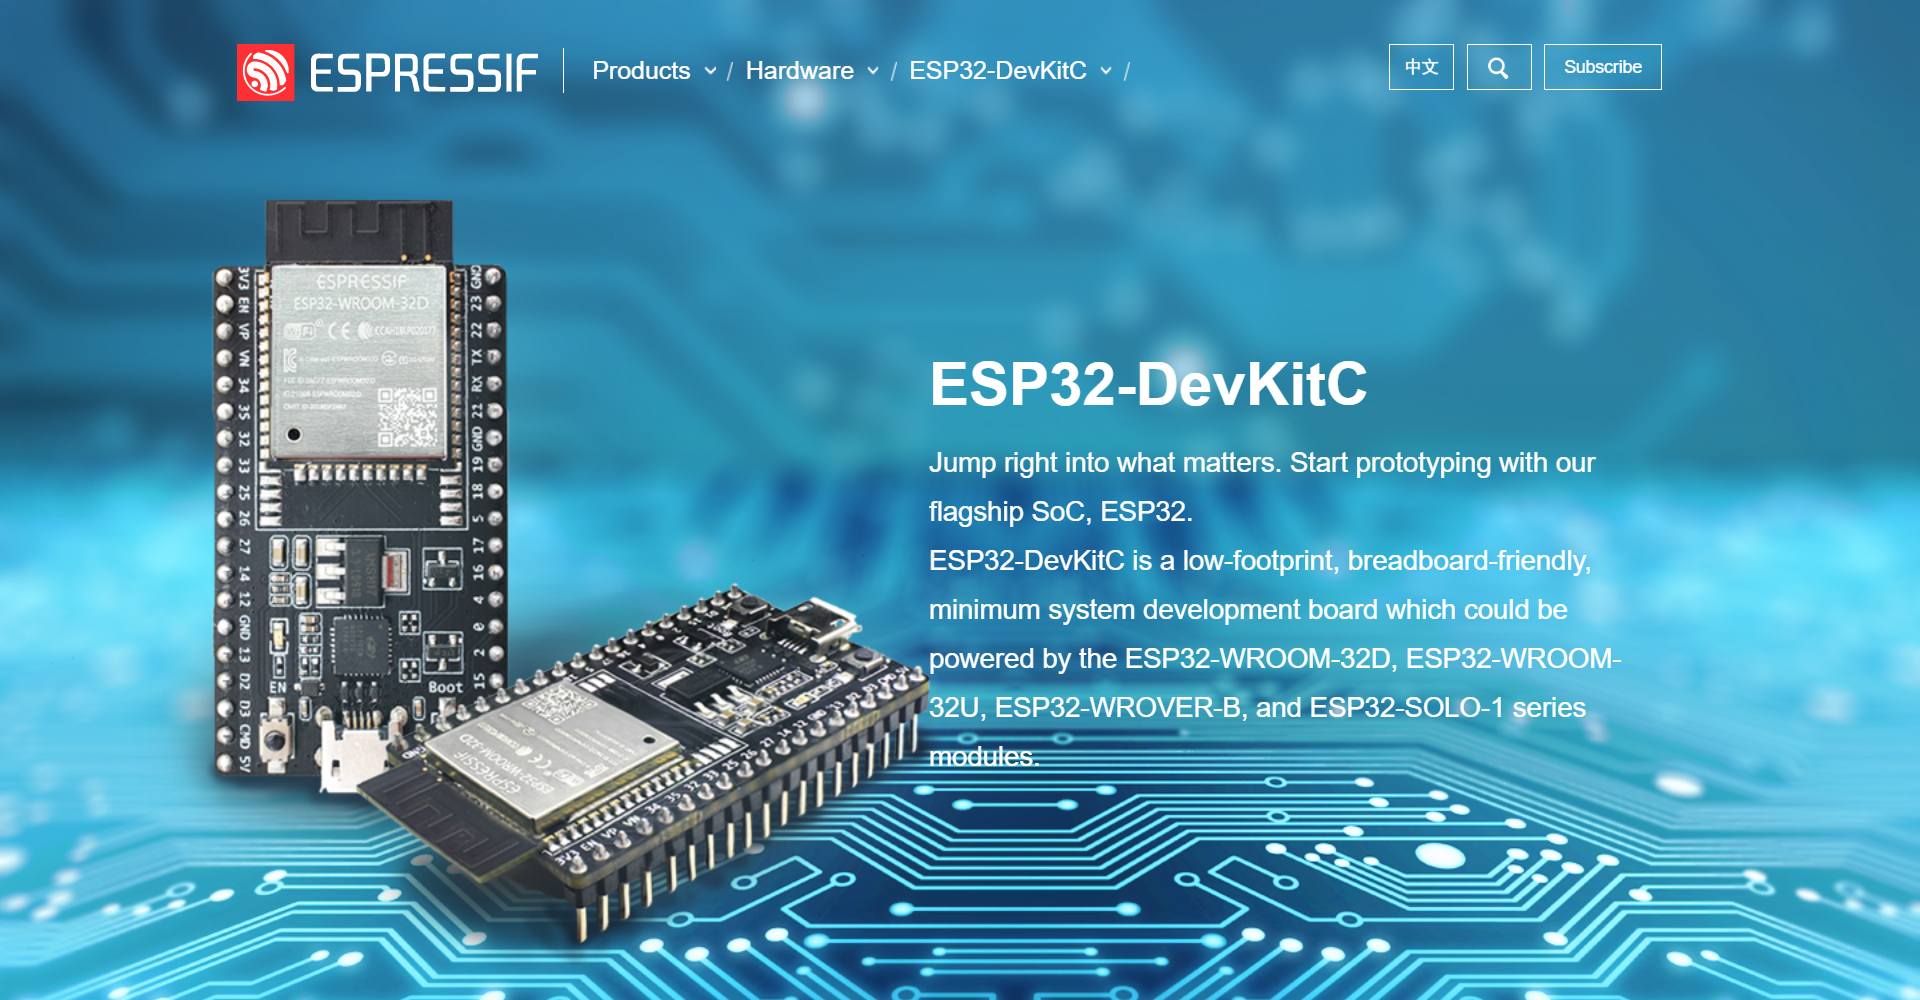
\includegraphics[width=.8\textwidth]{img/esp32-devkitc.png}\\
		\url{www.espressif.com/en/products/hardware/esp32-devkitc/overview}
	\end{center}
\end{frame}

\begin{frame}{Hardware used for the following examples}{Arduino Learning Kit Starter with ESP32 microcontroller}
	\begin{center}
		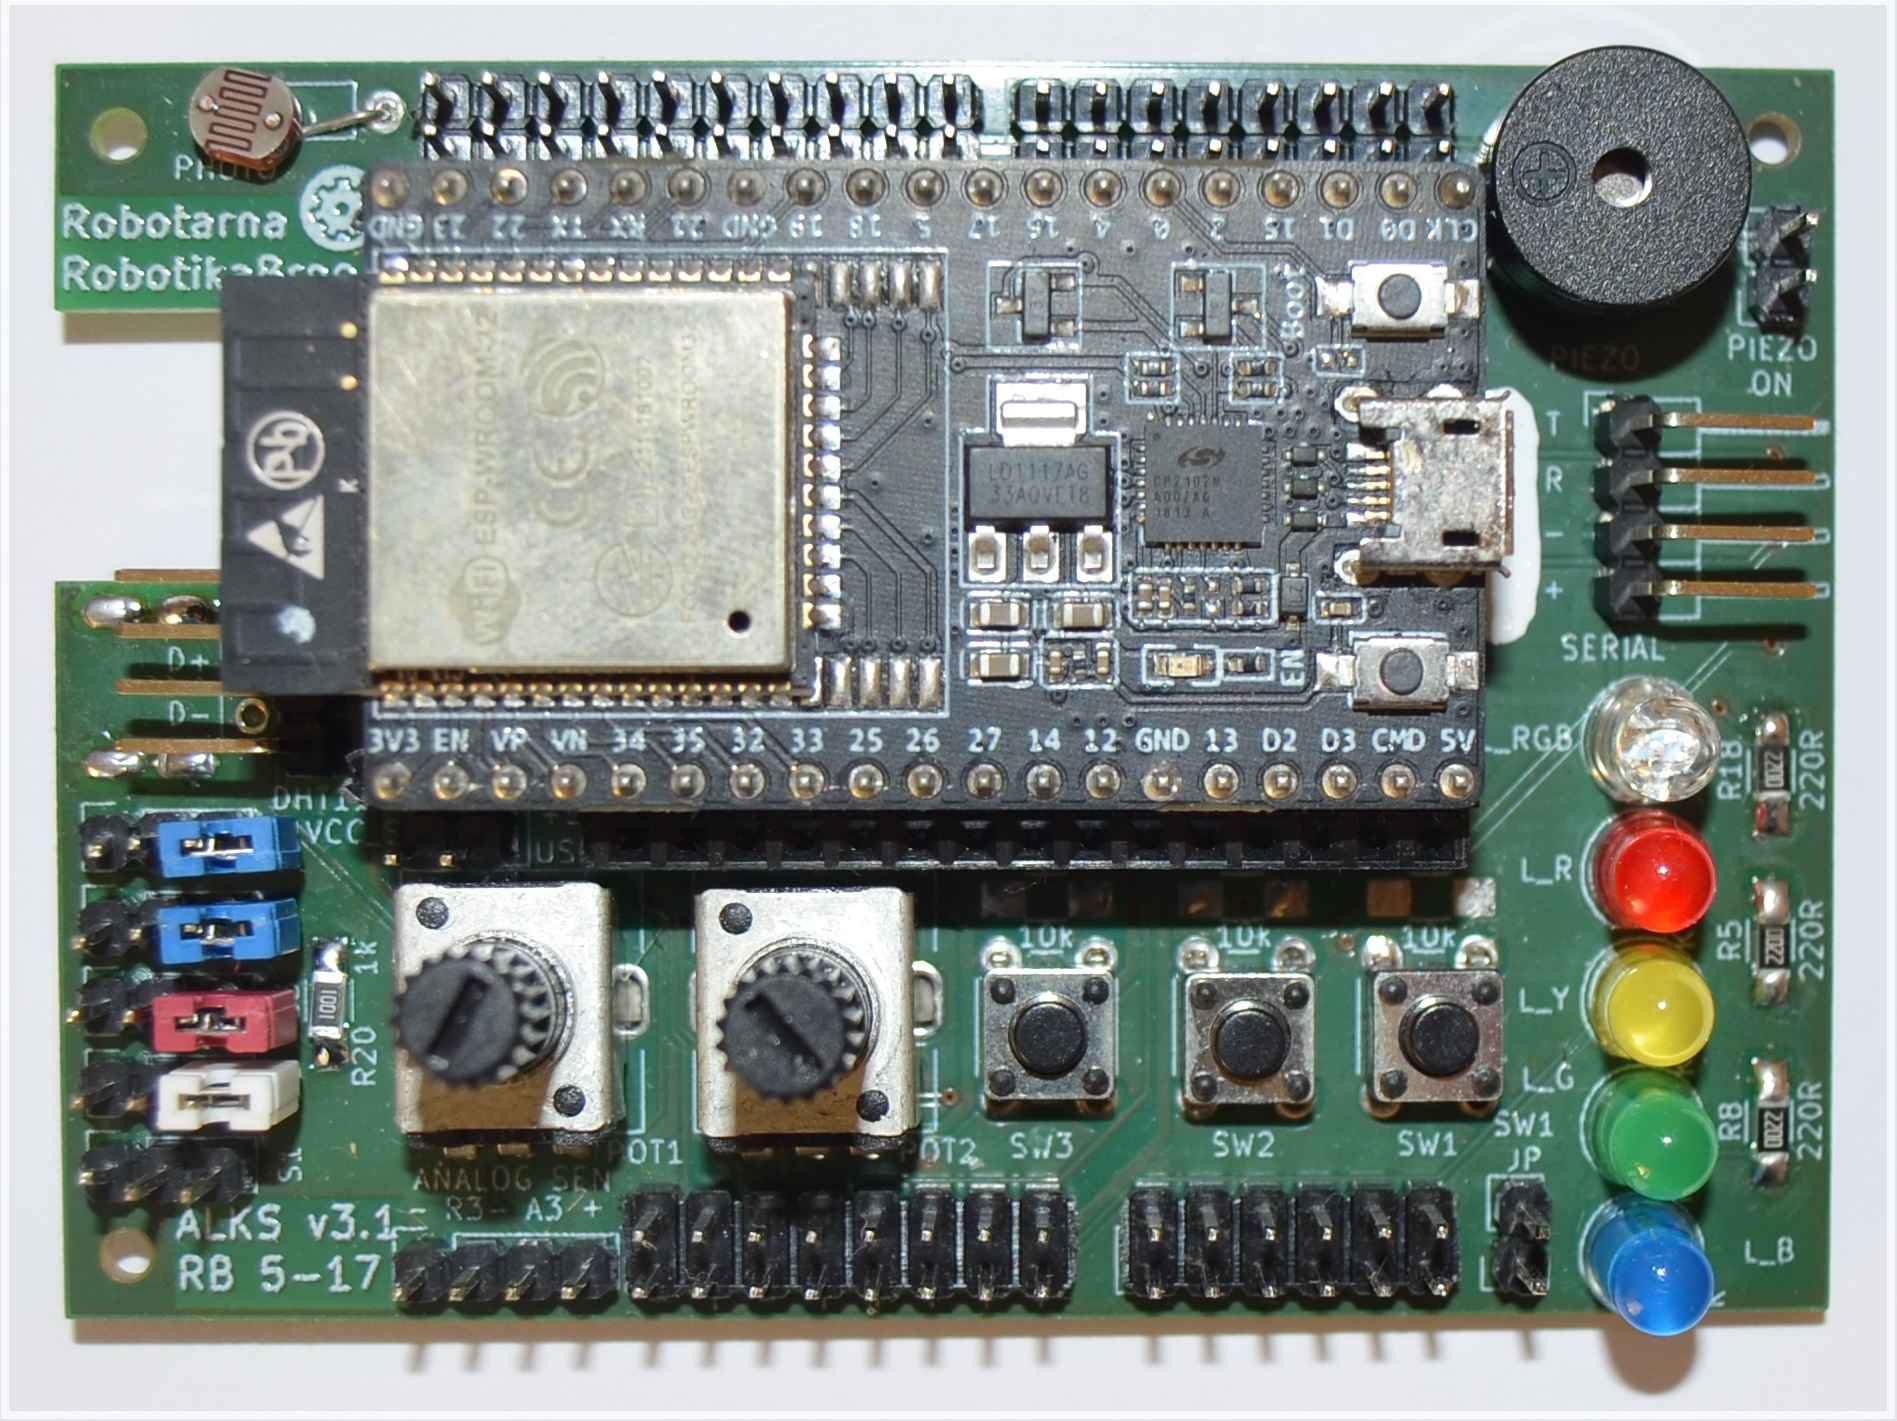
\includegraphics[width=.5\textwidth]{img/alks.jpg}\\
		\url{https://github.com/RoboticsBrno/ArduinoLearningKitStarter}
	\end{center}
\end{frame}

\begin{frame}{Hardware used for the following examples}{... connected to oscilloscope}
	\begin{center}
		\includegraphics[width=.6\textwidth]{img/scope.jpg}
	\end{center}
\end{frame}

\begin{frame}{How the oscilloscope works}
	\begin{block}{Presented in the video}
		\begin{itemize}
			\item Oscilloscope measures voltage with time
			\item It displays a graph (X axis = time; Y axis = voltage)
			\item Our FreeRTOS tasks control LEDs
			\item We can see which task is running = which LED is blinking
			\item Fast changes can be seen by the oscilloscope
		\end{itemize}
	\end{block}
\end{frame}

\begin{frame}{How the oscilloscope works}
	\begin{center}
		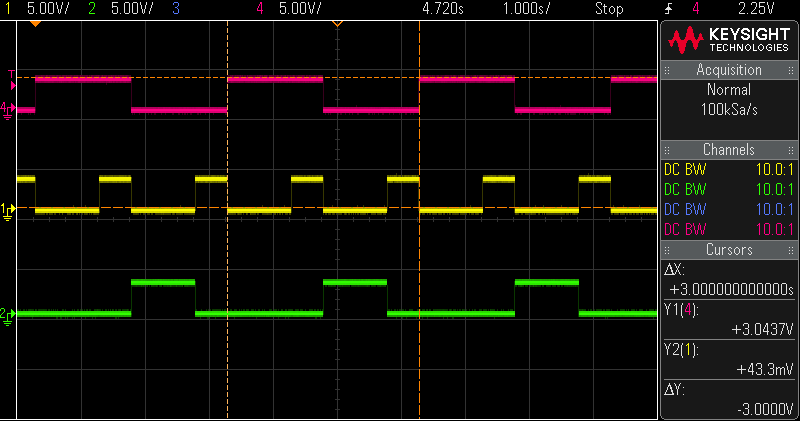
\includegraphics[width=.9\textwidth]{img/scopeTrafficLights.png}
	\end{center}
\end{frame}

\section[Minimal working example]{Minimal working example}

\begin{frame}{Overview}
	\tableofcontents[currentsection]
\end{frame}

%\begin{frame}{The used hardware -- ESP32}
%	\begin{center}
%		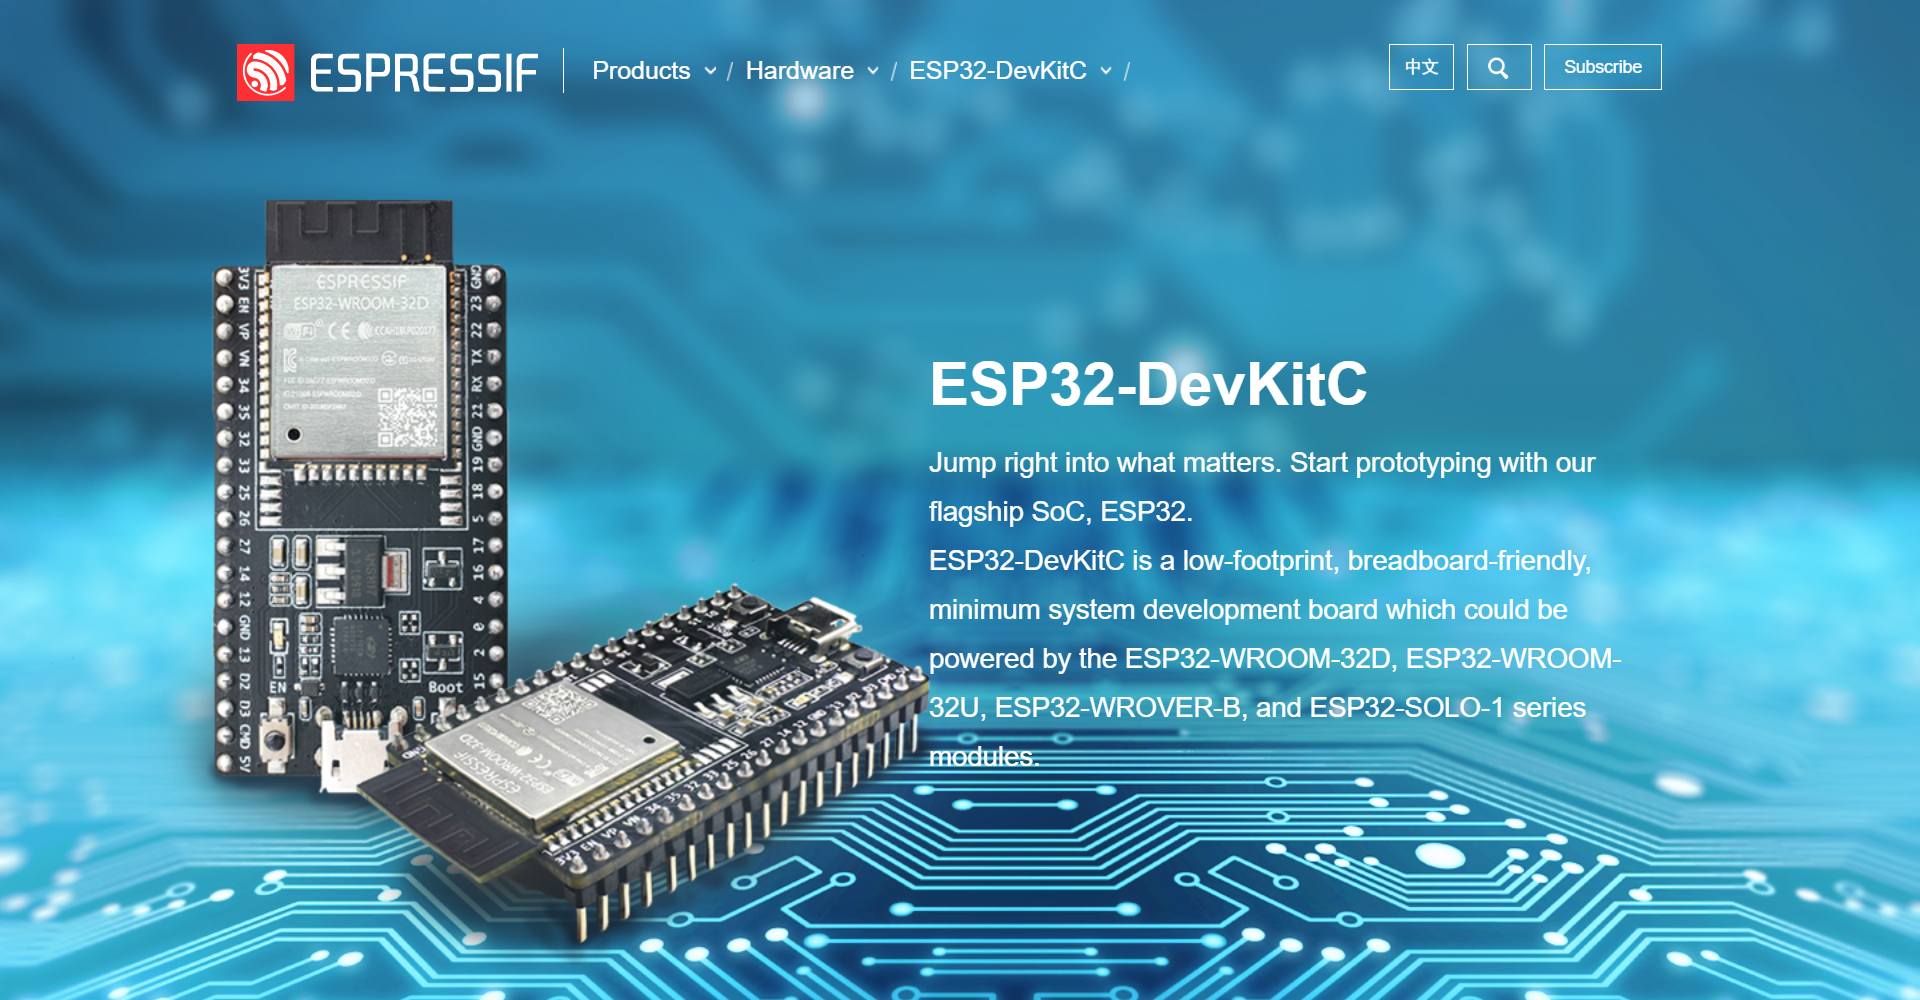
\includegraphics[width=.8\textwidth]{img/esp32-devkitc.png}\\
%		\url{https://docs.espressif.com/projects/esp-idf/}
%	\end{center}
%\end{frame}

\begin{frame}[fragile]{Minimal working example}
	\Cpp
	\begin{lstlisting}
#include <Arduino.h>

// called one time in the beginning
void setup() {
    pinMode(L_R, OUTPUT);    // Activate red LED
}

// repeats forever
void loop() {
    digitalWrite(L_R, HIGH); // Red LED on
    delay(1000);             // wait 1000 ms
    digitalWrite(L_R, LOW);  // Red LED off
    vTaskDelay(1000);        // wait 1000 scheduler ticks
}
	\end{lstlisting}
\end{frame}

\begin{frame}
	\begin{center}
		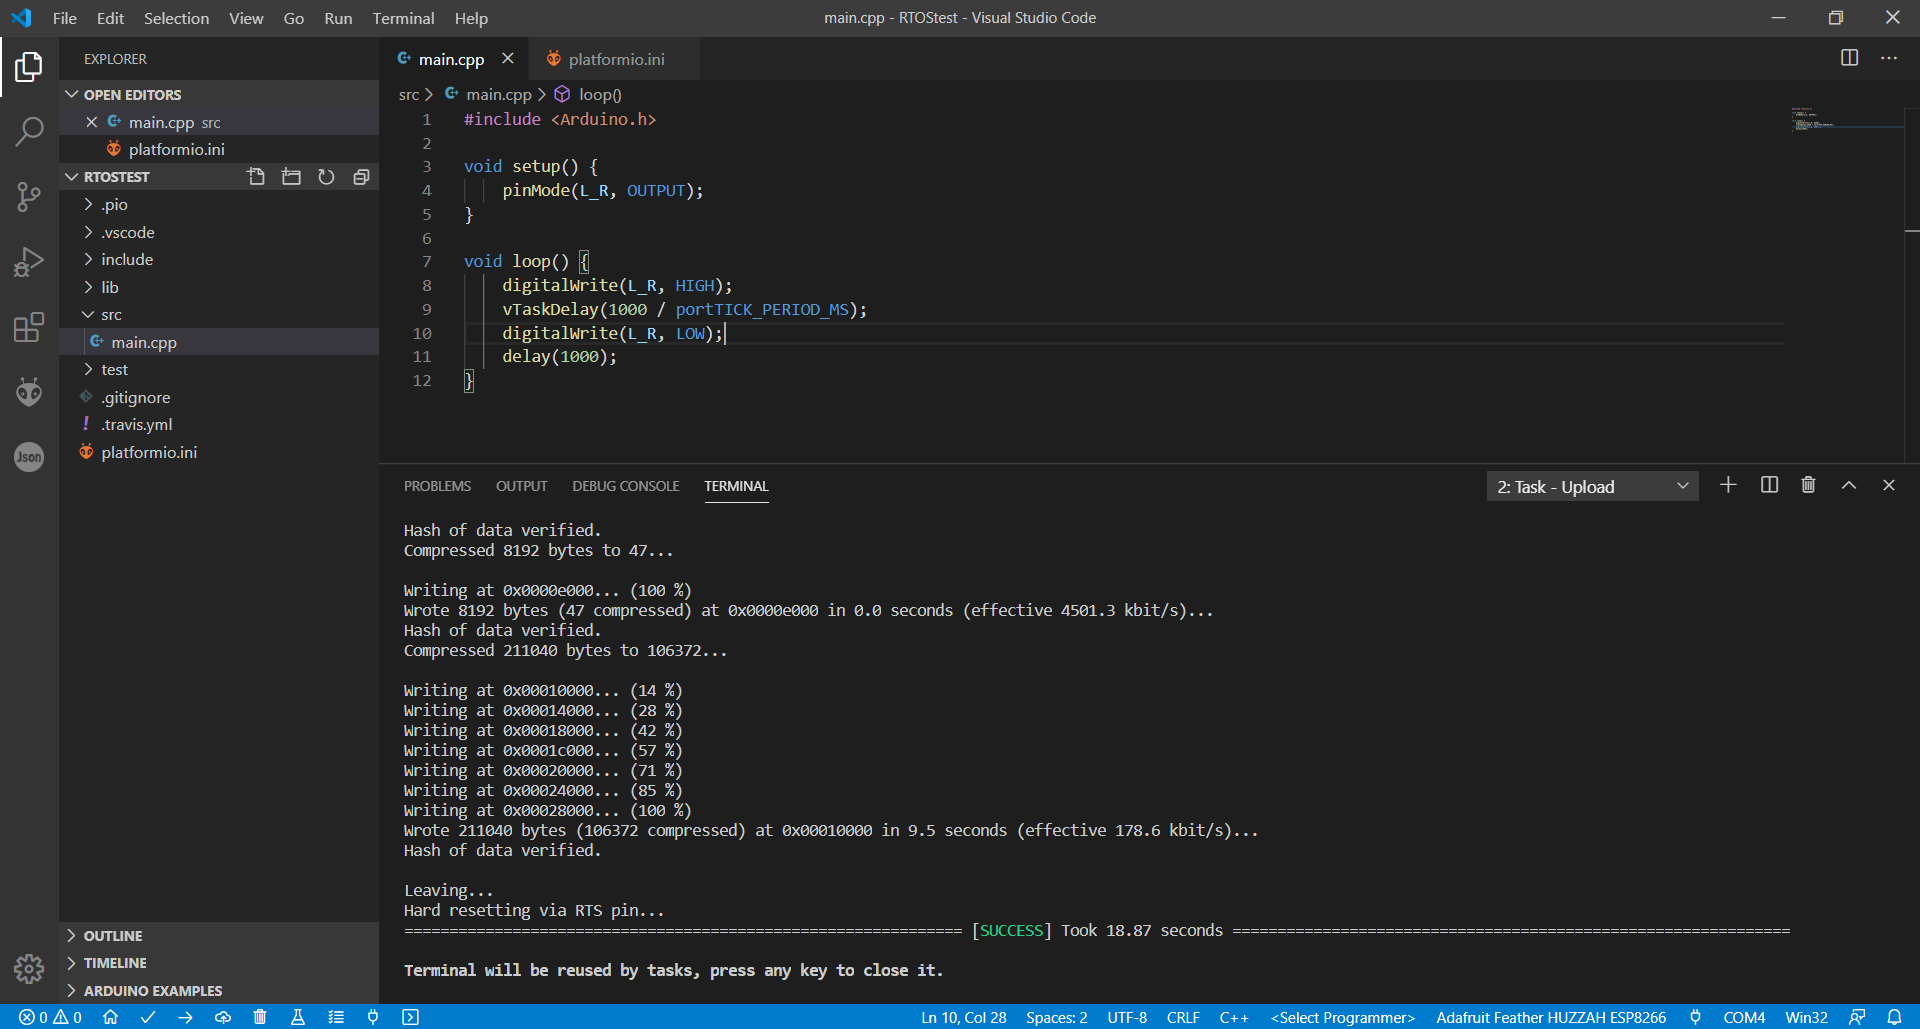
\includegraphics[width=\textwidth]{img/PlatformIOscreen.png}
	\end{center}
\end{frame}

\begin{frame}[fragile]{delay() vs. vTaskDelay()}
	\begin{center}
		\Cpp
		\begin{lstlisting}
// Busy wait for 1000 ms
delay(1000);
		\end{lstlisting}
		{\Large vs.}
		\Cpp
		\begin{lstlisting}
// Delay a task for a given number of RTOS ticks
vTaskDelay(1000);
		\end{lstlisting}
		{\Large vs.}
		\Cpp
		\begin{lstlisting}
// Delay a task for 1000 ms
vTaskDelay(1000 / portTICK_PERIOD_MS);
		\end{lstlisting}
		\url{https://www.freertos.org/a00127.html}
	\end{center}
\end{frame}

\begin{frame}{delay() vs. vTaskDelay()}
	\begin{center}
		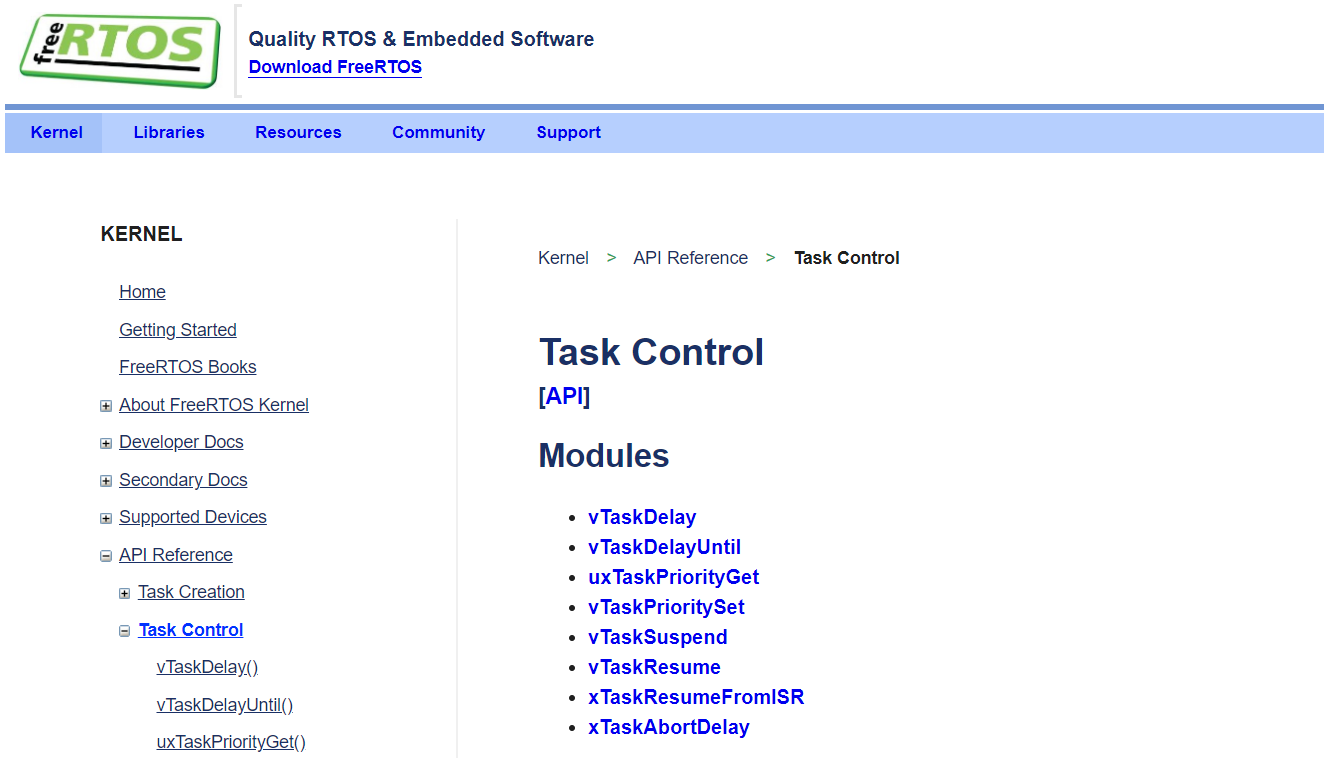
\includegraphics[width=.75\textwidth]{img/vTaskDelay.png}
		\url{https://www.freertos.org/a00127.html}
	\end{center}
\end{frame}

\begin{frame}[fragile]{Note: FreeRTOS naming convention}
	\Cpp
	\begin{lstlisting}
void vTaskDelay( const TickType_t xTicksToDelay );
BaseType_t xTaskCreate( ... );
	\end{lstlisting}
	
	\begin{itemize}
		\item \textbf{v} -- return type, here void
		\begin{itemize}
			\item [u] unsigned
			\item [l] long
			\item [s] short
			\item [c] char
			\item [p] pointer
			\item [x] variables of non stdint types
		\end{itemize}
		\item \textbf{TaskDelay} -- name in camel case
	\end{itemize}

	\vspace{0.5cm}
	\url{www.freertos.org/FreeRTOS-Coding-Standard-and-Style-Guide.html}
\end{frame}


\section[Tasks and jobs]{Tasks and jobs}
\subsection[New task creation]{New task creation}

\begin{frame}{Overview}
	\tableofcontents[currentsection]
\end{frame}

\begin{frame}[fragile]{New task creation}
	\begin{center}
		\Cpp
		\begin{lstlisting}
BaseType_t xTaskCreate(
	TaskFunction_t pvTaskCode, // Called function
	const char * const pcName, // Task name (string)
	configSTACK_DEPTH_TYPE usStackDepth, // Stack size
	void *pvParameters, // Parameters given to the task
	UBaseType_t uxPriority, // Priority of the task
	TaskHandle_t *pxCreatedTask // Task handle
);
		\end{lstlisting}
		\url{https://www.freertos.org/a00125.html}
	\end{center}
\end{frame}

\begin{frame}[fragile]{New task creation}{Imagine a function}
	\Cpp
	\begin{lstlisting}
void blinkLedForever(int led) {
	for(;;) {  // repeat forever
		digitalWrite(led, HIGH); // led on
		digitalWrite(led, LOW);  // led off
	}
}
	\end{lstlisting}
\end{frame}

\begin{frame}[fragile]
	\begin{center}
		\Cpp
		\begin{lstlisting}
void yellowTask(void * pvParameters) {
	blinkLedForever(L_Y);
}
	
void setup() {
	pinMode(L_Y, OUTPUT);
	xTaskCreate(
		yellowTask,   // Function to implement the task
		"Yellow task", // Name of the task
		10000,     // Stack size in words
		NULL,      // Task input parameter
		1,         // Priority of the task
		NULL       // Task handle.
	);
}
		\end{lstlisting}
	\end{center}
\end{frame}

\begin{frame}{New task creation}
	\begin{center}
		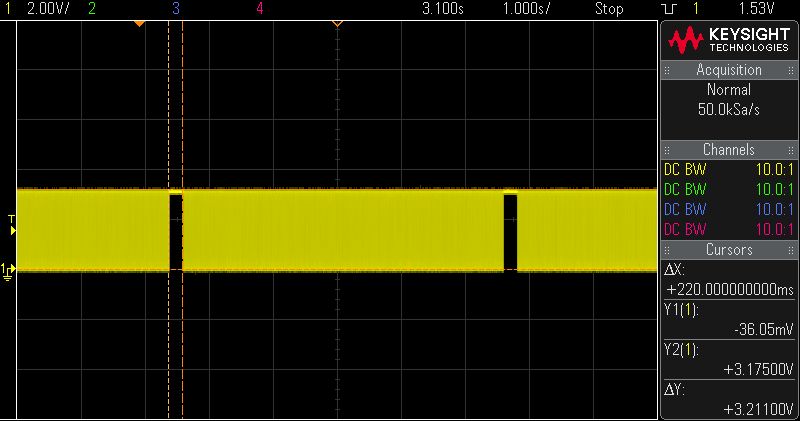
\includegraphics[width=.9\textwidth]{img/scope_1.png}
	\end{center}
\end{frame}

\begin{frame}{New task creation}
	\begin{center}
		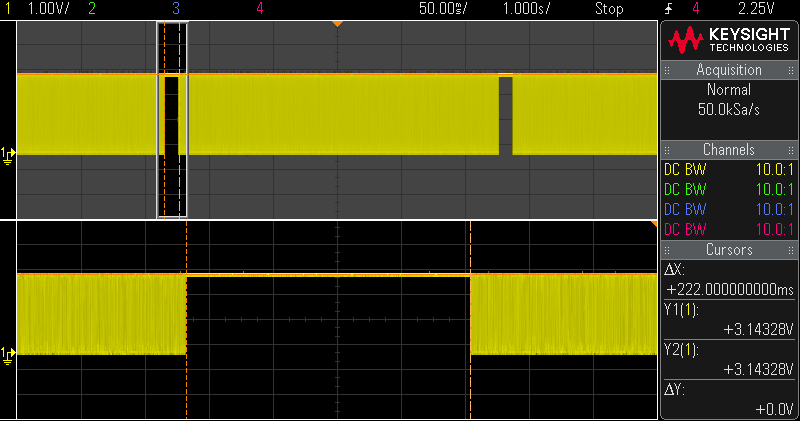
\includegraphics[width=.9\textwidth]{img/scope_1a.png}
	\end{center}
\end{frame}

\begin{frame}{New task creation}
	\begin{center}
		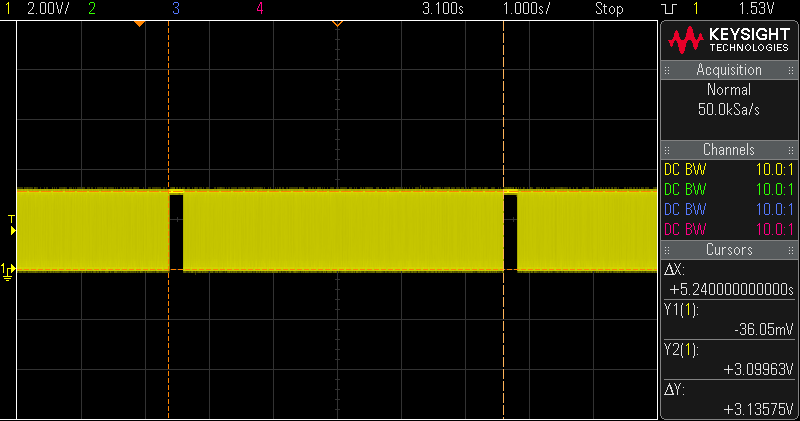
\includegraphics[width=.9\textwidth]{img/scope_1b.png}
	\end{center}
\end{frame}

\begin{frame}{New task creation}
	\begin{center}
		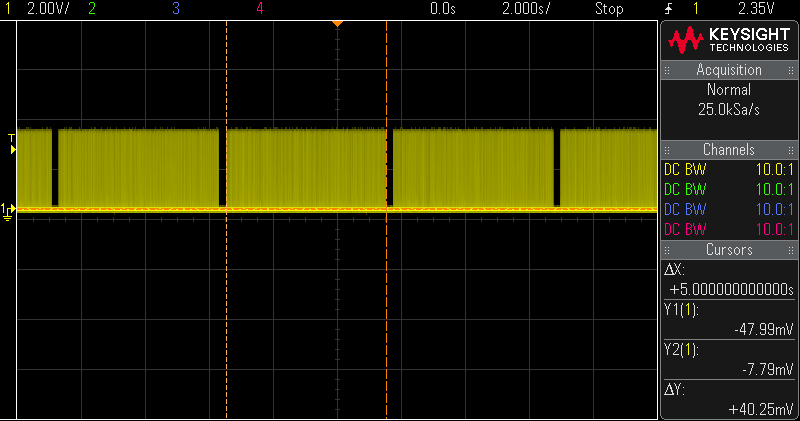
\includegraphics[width=.9\textwidth]{img/scope_1c.png}
	\end{center}
\end{frame}

\begin{frame}{New task creation}
	\begin{center}
		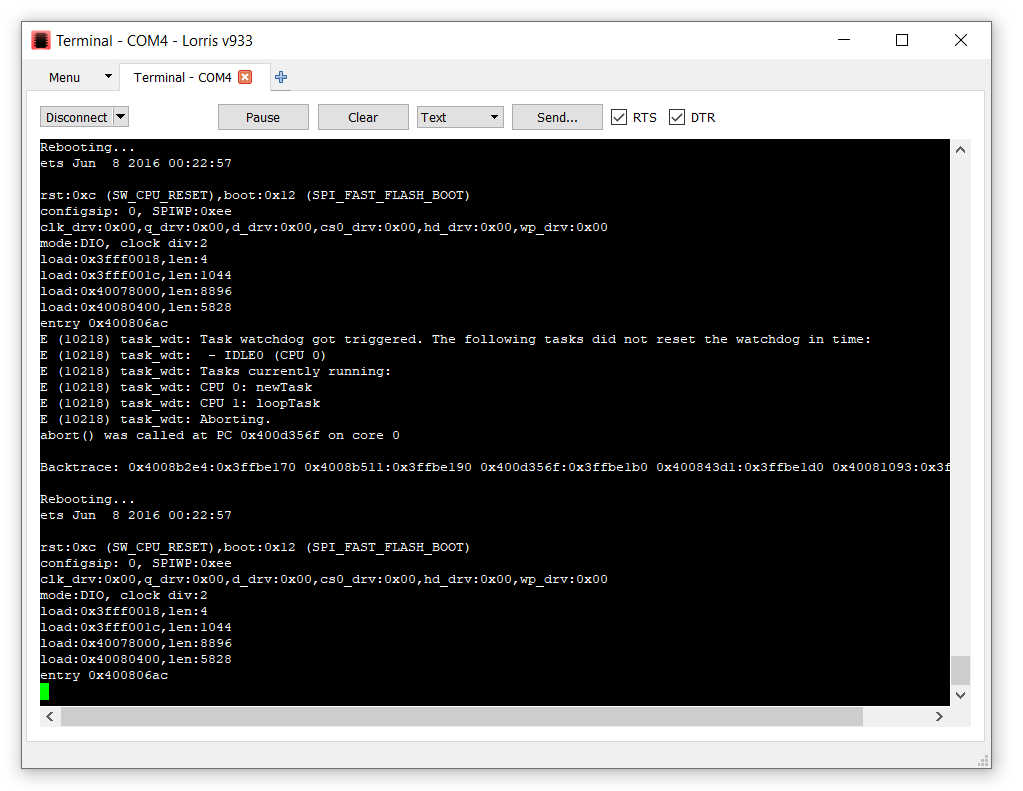
\includegraphics[width=.6\textwidth]{img/lorrisRebooting.png}
	\end{center}
\end{frame}

\begin{frame}{New task creation}
	\begin{block}{Single core}
		\begin{itemize}
			\item Scheduler is running on the same core.
			\item FreeRTOS has some watchdogs.
			\item If the scheduler (or task) does not trigger the watchdog on time, the watchdog resets the processor.
			\item Watchdog can be disabled (not recommended).
		\end{itemize}
	\end{block}
	\begin{center}\Large vs.\end{center}
	\begin{block}{Multi core}
		\begin{itemize}
			\item One task can occupy the whole core.
			\item There must be a reserved space for the scheduler at one core.
			\item Keep in mind the watchdogs.
		\end{itemize}
	\end{block}
\end{frame}

\begin{frame}[fragile]{A task with waiting}
	\Cpp
	\begin{lstlisting}
void blinkLedForeverWithDelay(int led, uint32_t ticks) {
	for(;;) {
		digitalWrite(led, HIGH);
		vTaskDelay(ticks);
		digitalWrite(led, LOW);
		vTaskDelay(ticks);
	}
}
	\end{lstlisting}
\end{frame}

\begin{frame}[fragile]{A task with waiting}
	\Cpp
	\begin{lstlisting}
void redTask(void * pvParameters) {
	blinkLedForeverWithDelay(L_R, 5 /*ms*/);
}
	
void setup() {
	esp_task_wdt_deinit();
	pinMode(L_R, OUTPUT);
	xTaskCreate(redTask, "redTask", 10000, NULL, 1, NULL);
}
	\end{lstlisting}
\end{frame}

\begin{frame}{A task with waiting}
	\begin{center}
		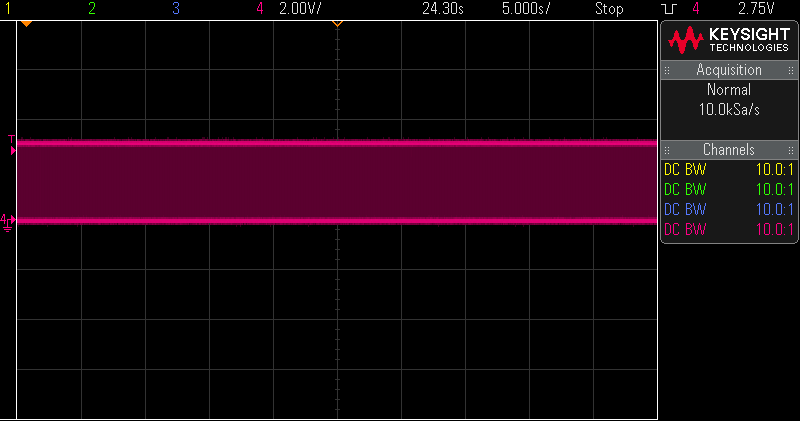
\includegraphics[width=.9\textwidth]{img/scope_2.png}
	\end{center}
\end{frame}

\begin{frame}{A task with waiting}
	\begin{center}
		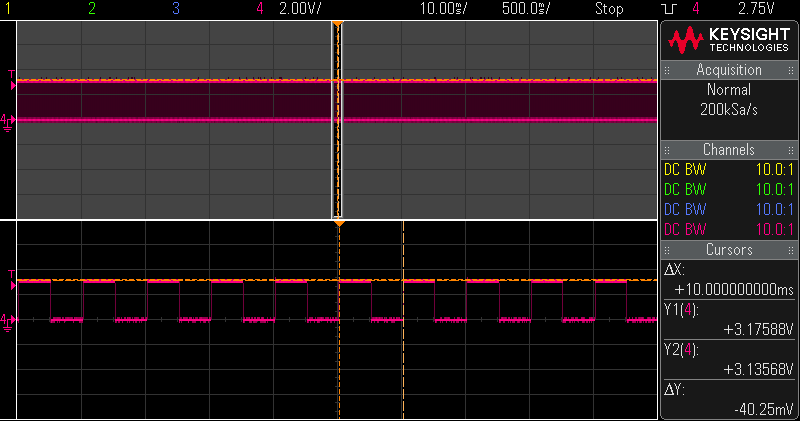
\includegraphics[width=.9\textwidth]{img/scope_3.png}
	\end{center}
\end{frame}

\begin{frame}{The very very common mistakes}
	\begin{block}{Do not forget to reserve a time for scheduler and context switching!}
		\begin{itemize}
			\item Your tasks are interrupted when the scheduler is running.
			\item Context switching consumes time, too.
		\end{itemize}
	\end{block}

	\begin{block}{Do not forget the watch dogs!}
		\begin{itemize}
			\item The CPU resets easily hide themselves behind the periodic tasks.
		\end{itemize}
	\end{block}

	\begin{block}{Do not forget the main task!}
		\begin{itemize}
			\item If the main() function is still running, it is a task, too.
		\end{itemize}
	\end{block}
\end{frame}

\subsection[Task properties]{Task properties}

\begin{frame}{Overview}
	\tableofcontents[currentsection]
\end{frame}

\begin{frame}{Task management}
	\begin{block}{Changes from the previous example}
		\begin{itemize}
			\item Yellow task is pinned to Core 1.
			\item The scheduler is running on the Core 0.
			\item The task watch dog is disabled.
		\end{itemize}
	\end{block}
\end{frame}

\begin{frame}[fragile]{Remember previous functions}
	\begin{center}
		\Cpp
		\begin{lstlisting}
void blinkLedForever(int led) {
	for(;;) {  // repeat forever
		digitalWrite(led, HIGH); // led on
		digitalWrite(led, LOW);  // led off
	}
}

void yellowTask(void * pvParameters) {
	blinkLedForever(L_Y);
}
		\end{lstlisting}
	\end{center}
\end{frame}

\begin{frame}[fragile]
	\begin{center}
		\Cpp
		\begin{lstlisting}		
void setup() {
	esp_task_wdt_deinit();
	pinMode(L_Y, OUTPUT);
		
	xTaskCreatePinnedToCore(
		yellowTask,   // Function to implement the task
		"yellowTask", // Name of the task
		10000,     // Stack size in words
		NULL,      // Task input parameter
		2,         // Priority of the task
		NULL,       // Task handle.
		1  // CPU core ID
	);
}
		\end{lstlisting}
	\end{center}
\end{frame}

\begin{frame}{Task management}
	\begin{center}
		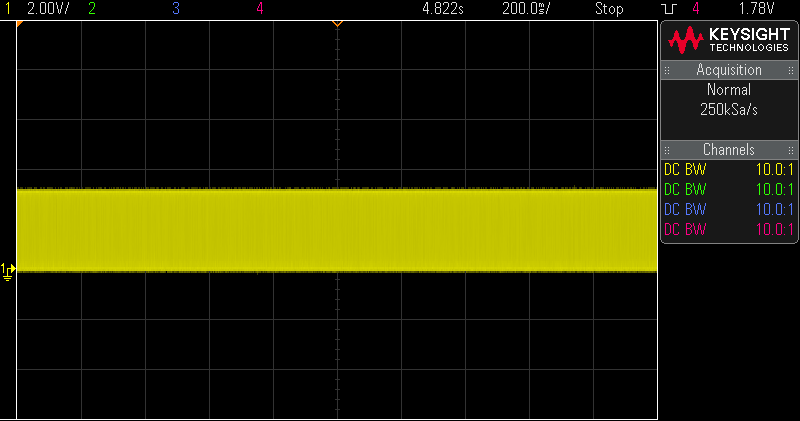
\includegraphics[width=.9\textwidth]{img/scope_4.png}
	\end{center}
\end{frame}

\begin{frame}{Task management}
	\begin{center}
		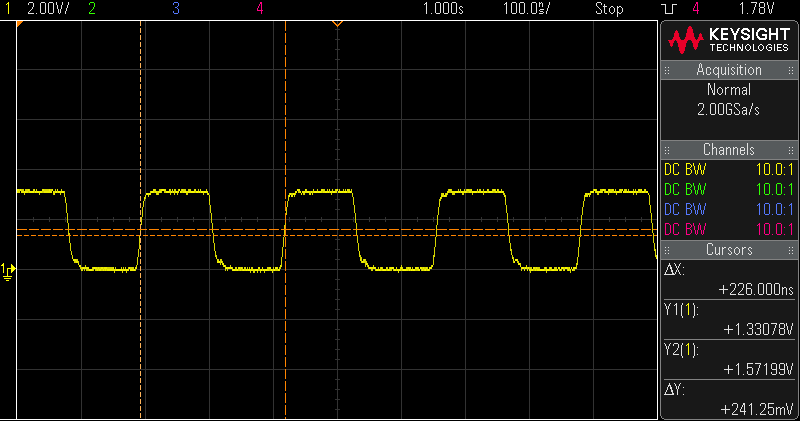
\includegraphics[width=.9\textwidth]{img/scope_4a.png}
	\end{center}
\end{frame}

\begin{frame}{Task management}
	\begin{center}
		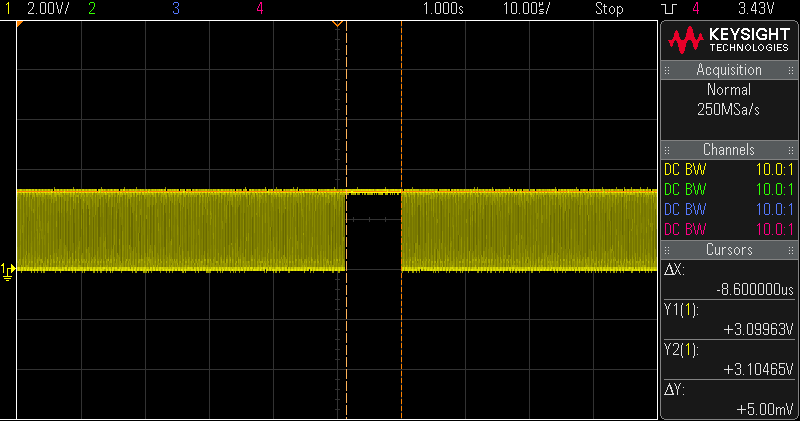
\includegraphics[width=.9\textwidth]{img/scope_4b.png}
	\end{center}
\end{frame}

\begin{frame}{Task management}
	\begin{center}
		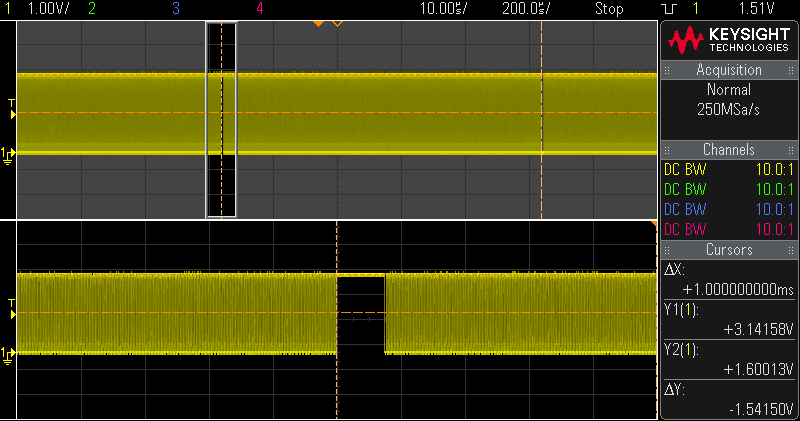
\includegraphics[width=.9\textwidth]{img/scope_4c.png}
	\end{center}
\end{frame}

\begin{frame}{Task management}
	\begin{center}
		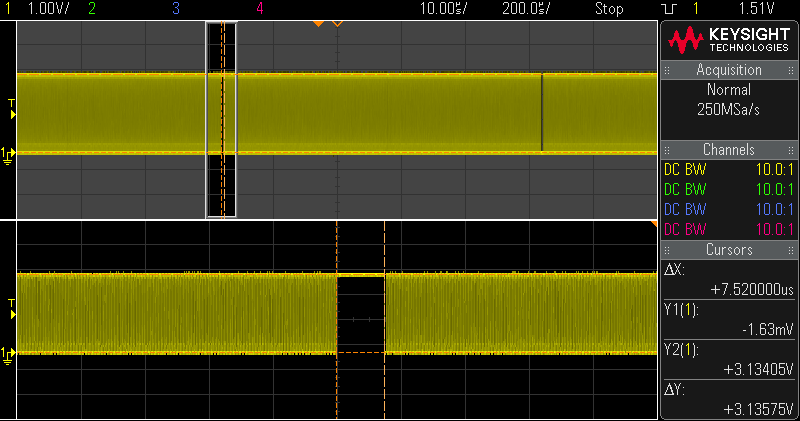
\includegraphics[width=.9\textwidth]{img/scope_4d.png}
	\end{center}
\end{frame}

\begin{frame}{Task management}
	\begin{center}
		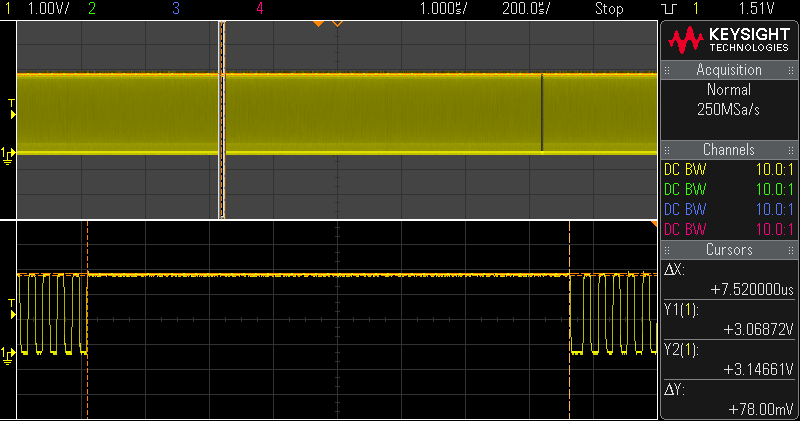
\includegraphics[width=.9\textwidth]{img/scope_4e.png}
	\end{center}
\end{frame}

\begin{frame}{Task management}
	\begin{block}{Properties of the task}
		\begin{itemize}
			\item The task is interrupted by the scheduler and by defined SW or HW interrupts.
			\item If we want to run an uninterrupted thread on the CPU core,\\do not use RTOS on this CPU core.
		\end{itemize}
	\end{block}
\end{frame}

\subsection[Multiple tasks]{Multiple tasks}

\begin{frame}{Overview}
	\tableofcontents[currentsection]
\end{frame}

\begin{frame}[fragile]{Multiple tasks}{Warning: the watchdog will reset the CPU in this example}
	\begin{center}
		\Cpp
		\begin{lstlisting}
void redTask(void * pvParameters) {
	blinkLedForever(L_R);
}

void yellowTask(void * pvParameters) {
	blinkLedForever(L_Y);
}

void greenTask(void * pvParameters) {
	blinkLedForever(L_G);
}
		\end{lstlisting}
	\end{center}
\end{frame}

\begin{frame}[fragile]
	\begin{center}
		\Cpp
		\begin{lstlisting}
void setup() {
	esp_task_wdt_deinit();
	pinMode(L_R, OUTPUT);
	pinMode(L_Y, OUTPUT);
	pinMode(L_G, OUTPUT);
	
	xTaskCreate(redTask, "redTask", 10000, NULL, 1, NULL);
	xTaskCreate(yellowTask,"yellowTask",10000,NULL,1,NULL);
	blinkLedForever(L_G);
}
		\end{lstlisting}
	\end{center}
\end{frame}

\begin{frame}{Multiple tasks}
	\begin{center}
		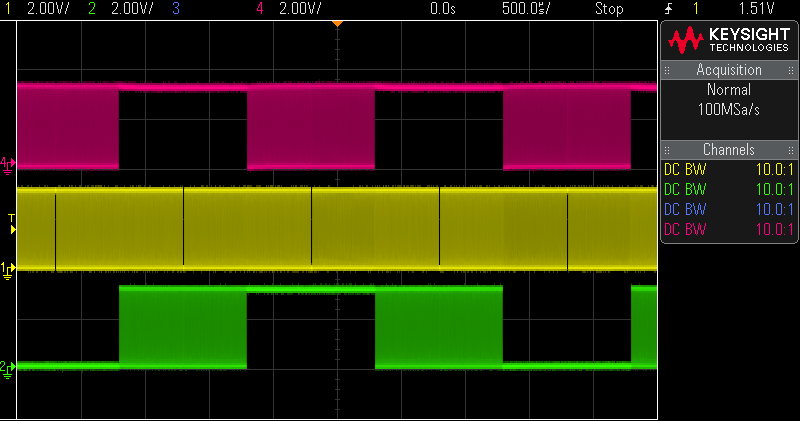
\includegraphics[width=.9\textwidth]{img/scope_5.png}
	\end{center}
\end{frame}

\begin{frame}[fragile]{Now let's change the task priorities}
	\begin{center}
		\Cpp
		\begin{lstlisting}
(...)
xTaskCreate(redTask, "redTask", 10000, NULL, 2, NULL);
xTaskCreate(yellowTask,"yellowTask",10000,NULL,3,NULL);
blinkLedForever(L_G);
(...)
		\end{lstlisting}
	\end{center}
\end{frame}

\begin{frame}{Multiple tasks}
	\begin{center}
		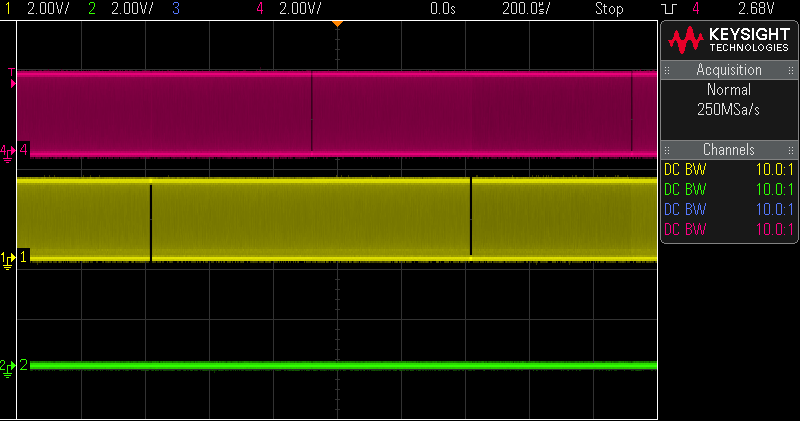
\includegraphics[width=.9\textwidth]{img/scope_5a.png}
	\end{center}
\end{frame}

\begin{frame}[fragile]{Now let's change the task priorities}
	\begin{center}
		\Cpp
		\begin{lstlisting}
(...)
xTaskCreate(redTask, "redTask", 10000, NULL, 0, NULL);
xTaskCreate(yellowTask,"yellowTask",10000,NULL,0,NULL);
blinkLedForever(L_G);
(...)
		\end{lstlisting}
	\end{center}
\end{frame}

\begin{frame}{Multiple tasks}
	\begin{center}
		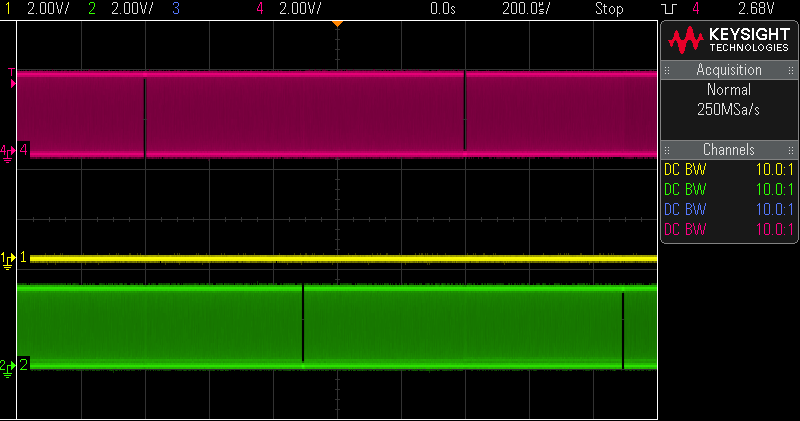
\includegraphics[width=.9\textwidth]{img/scope_5b.png}
	\end{center}
\end{frame}

\subsection[Jobs]{Jobs}

\begin{frame}{Overview}
	\tableofcontents[currentsection]
\end{frame}

\begin{frame}[fragile]{Tasks and jobs}{Imagine a function}
	\begin{center}
		\Cpp
		\begin{lstlisting}
void blinkLedForTime(uint8_t led,
                            uint64_t run_us,
                            uint64_t wait_ms) {
	for(;;) {
		// Blinking for specified time in microseconds
		for(uint64_t t = micros(); t + run_us > micros();) {
			digitalWrite(led, HIGH);
			digitalWrite(led, LOW);
		}
		vTaskDelay(wait_ms);
	}
}
		\end{lstlisting}
	\end{center}
\end{frame}

\begin{frame}[fragile]
	\begin{center}
		\Cpp
		\begin{lstlisting}
blinkLedForTime(L_G, 300, 1);
		\end{lstlisting}
		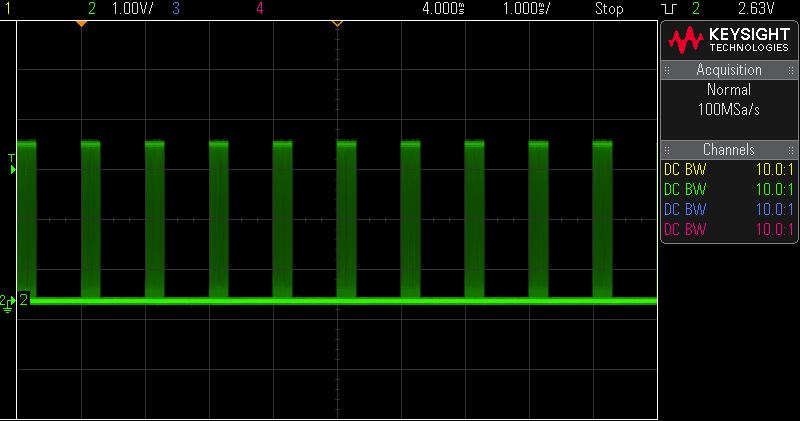
\includegraphics[width=.9\textwidth]{img/scope_6a.png}
	\end{center}
\end{frame}

\begin{frame}[fragile]
	\begin{center}
		\Cpp
		\begin{lstlisting}
blinkLedForTime(L_G, 300, 1);
		\end{lstlisting}
		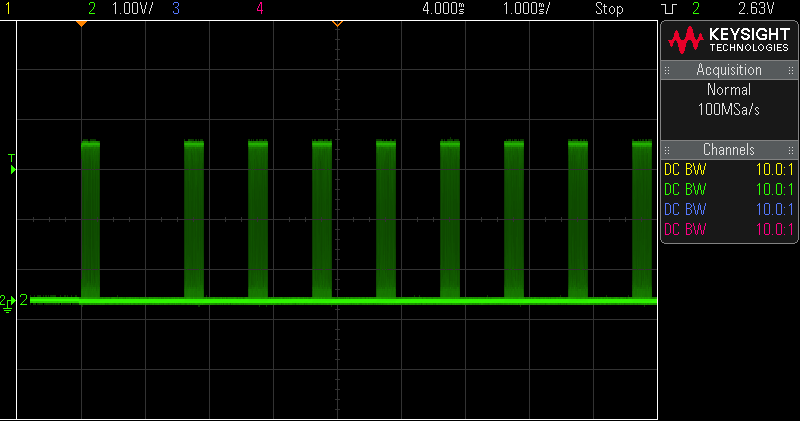
\includegraphics[width=.9\textwidth]{img/scope_6b.png}
	\end{center}
\end{frame}

\begin{frame}[fragile]
	\begin{center}
		\Cpp
		\begin{lstlisting}
blinkLedForTime(L_G, 900, 1);
		\end{lstlisting}
		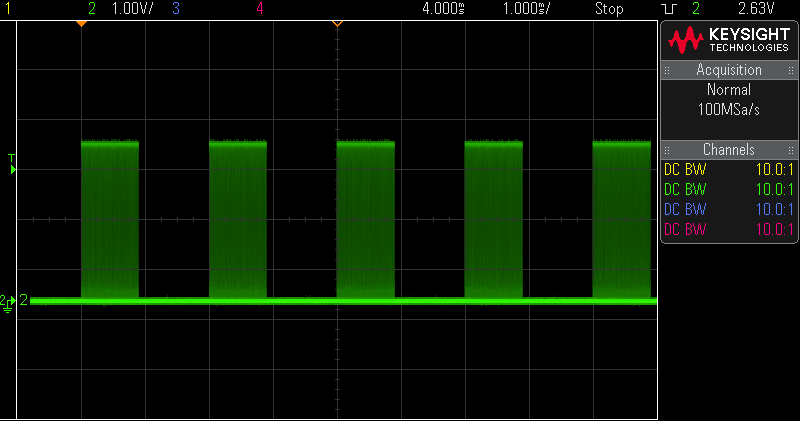
\includegraphics[width=.9\textwidth]{img/scope_6c.png}
	\end{center}
\end{frame}

\begin{frame}[fragile]
	\begin{center}
		\Cpp
		\begin{lstlisting}
blinkLedForTime(L_G, 900, 1);
		\end{lstlisting}
		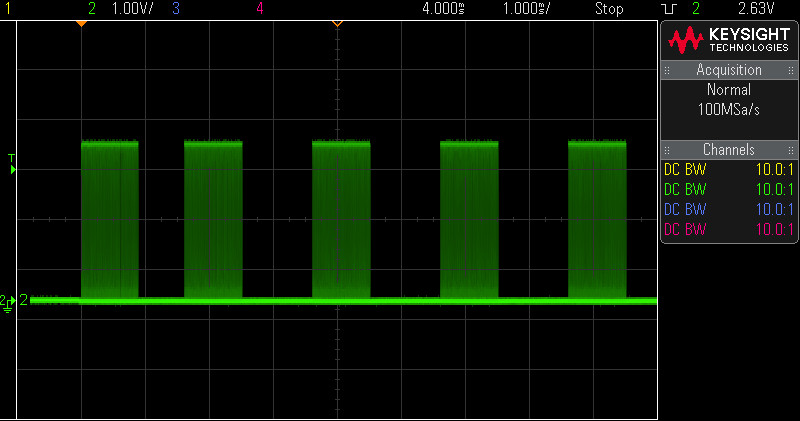
\includegraphics[width=.9\textwidth]{img/scope_6d.png}
	\end{center}
\end{frame}

\begin{frame}[fragile]
	\begin{center}
		\Cpp
		\begin{lstlisting}
blinkLedForTime(L_G, 1500, 2);
		\end{lstlisting}
		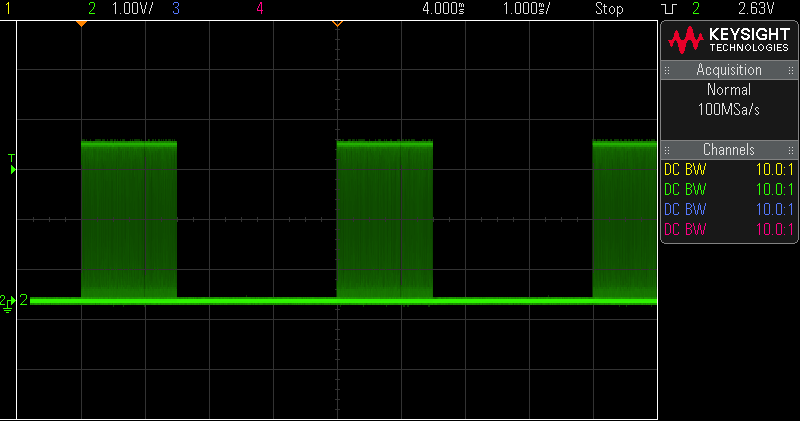
\includegraphics[width=.9\textwidth]{img/scope_6e.png}
	\end{center}
\end{frame}

\begin{frame}[fragile]
	\begin{center}
		\Cpp
		\begin{lstlisting}
blinkLedForTime(L_G, 1500, 1);
		\end{lstlisting}
		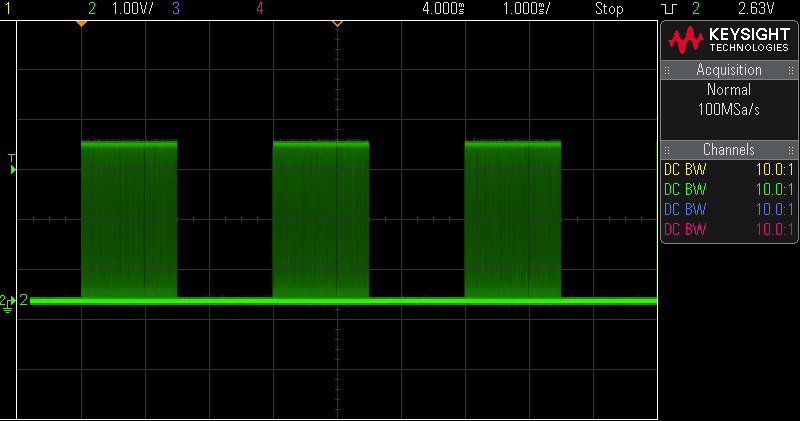
\includegraphics[width=.9\textwidth]{img/scope_6f.png}
	\end{center}
\end{frame}

\begin{frame}[fragile]
	\begin{center}
		\Cpp
		\begin{lstlisting}
blinkLedForTime(L_G, 1488, 1);
		\end{lstlisting}
		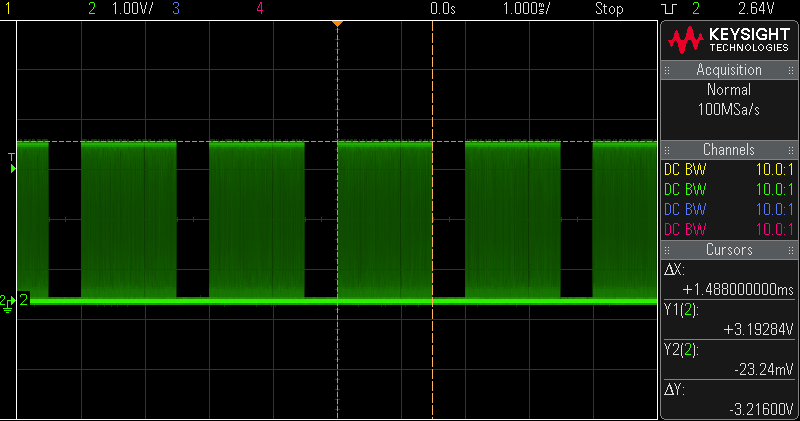
\includegraphics[width=.9\textwidth]{img/scope_6g.png}
	\end{center}
\end{frame}

\begin{frame}[fragile]
	\begin{center}
		\Cpp
		\begin{lstlisting}
blinkLedForTime(L_G, 1489, 1);
		\end{lstlisting}
		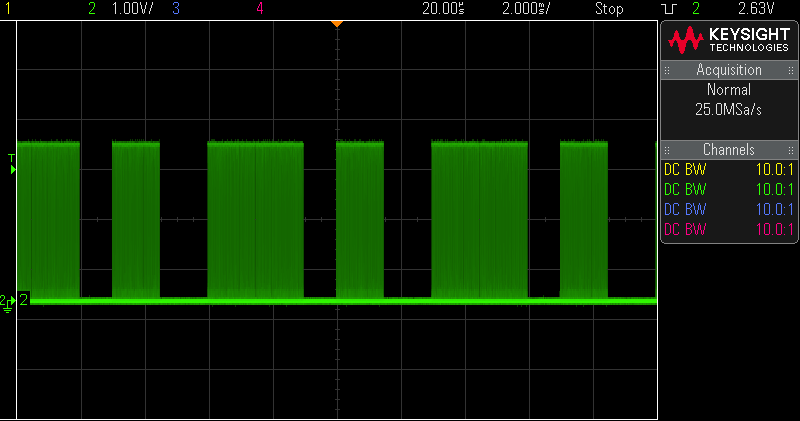
\includegraphics[width=.9\textwidth]{img/scope_6h.png}
	\end{center}
\end{frame}

\begin{frame}[fragile]
	\begin{center}
		\Cpp
		\begin{lstlisting}
blinkLedForTime(L_G, 1490, 1);
		\end{lstlisting}
		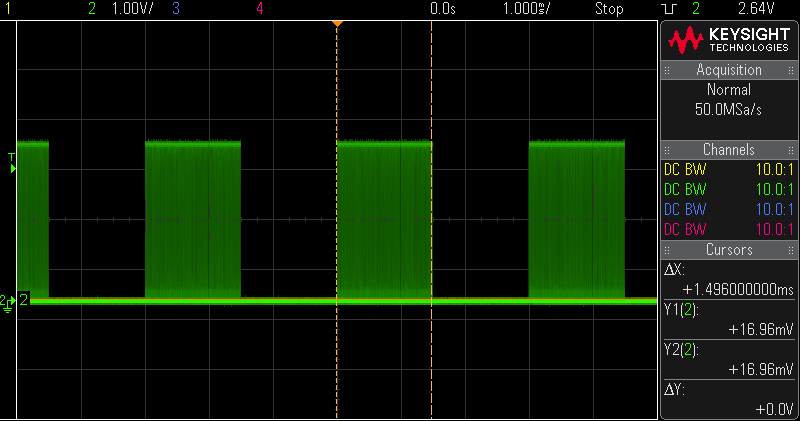
\includegraphics[width=.9\textwidth]{img/scope_6i.png}
	\end{center}
\end{frame}

\begin{frame}[fragile]{3 periodic tasks on 2 CPU cores}
	\begin{center}
		\Cpp
		\begin{lstlisting}
void redTask(void * pvParameters) {
	blinkLedForTime(L_R, 300, 1);
}

void yellowTask(void * pvParameters) {
	blinkLedForTime(L_Y, 300, 1);
}

void setup() {
(...)
	xTaskCreate(redTask,"redTask",10000,NULL,3,NULL,0);
	xTaskCreate(yellowTask,"yellowTask",10000,NULL,2,NULL,0);
	blinkLedForTime(L_G, 300, 1);
}
		\end{lstlisting}
	\end{center}
\end{frame}

\begin{frame}{3 periodic tasks on 2 CPU cores}
	\begin{center}
		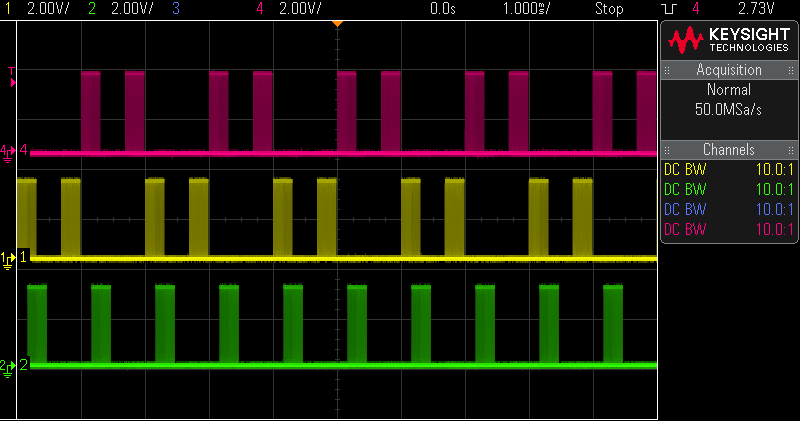
\includegraphics[width=.9\textwidth]{img/scope_7a.png}
	\end{center}
\end{frame}

\begin{frame}{Task control functions}
	\begin{itemize}
		\item xTaskCreate(...)
		\item xTaskCreatePinnedToCore(...)
		\item vTaskDelete(...)
		\item vTaskDelay(...)
		\item xTaskDelayUntil(...)
		\item vTaskSuspend(...)
		\item vTaskResume(...)
		\item taskYIELD()
		\item ...
	\end{itemize}
\end{frame}

\subsection[Timers]{Timers}

\begin{frame}{Overview}
	\tableofcontents[currentsection]
\end{frame}

\begin{frame}[fragile]{Timers}
	\begin{itemize}
		\item Good for periodic tasks
		\item Limited number of hardware timers
		\item \url{https://www.freertos.org/RTOS-software-timer.html}
	\end{itemize}

	\begin{center}
		\Cpp
		\begin{lstlisting}
TimerHandle_t xTimerCreate(
	const char * const pcTimerName,
	const TickType_t xTimerPeriod,
	const UBaseType_t uxAutoReload,
	void * const pvTimerID,
	TimerCallbackFunction_t pxCallbackFunction
);
		\end{lstlisting}
	\end{center}
\end{frame}

\begin{frame}[fragile]{Timers}
	\begin{center}
		\Cpp
		\begin{lstlisting}
void vTimerCallback(TimerHandle_t xTimer) {
	blinkLedOnce(L_Y, 1600);
}

void setup() {
	pinMode(L_Y, OUTPUT);
	TimerHandle_t xTimer = xTimerCreate(
		"Timer1", 2, pdTRUE, ( void * ) 0, vTimerCallback
	);
	xTimerStart(xTimer, 0);
}
		\end{lstlisting}
	\end{center}
\end{frame}

\begin{frame}{Timers}
	\begin{center}
		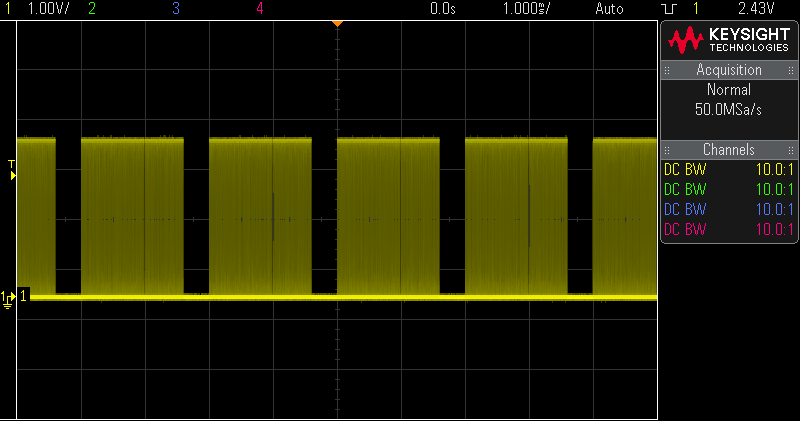
\includegraphics[width=.9\textwidth]{img/scope_8.png}
	\end{center}
\end{frame}

\section[Sharing data among threads]{Sharing data among threads}

\subsection[Critical sections]{Critical sections}

\begin{frame}{Overview}
	\tableofcontents[currentsection]
\end{frame}

\begin{frame}[fragile]{Imagine a function}
	\begin{center}
		\Cpp
		\begin{lstlisting}
void blinkLedForTimeCritical(
	uint8_t led, uint64_t run_us,
	uint64_t wait_ms, portMUX_TYPE *myMutex
) {
	for(;;) {
//		portENTER_CRITICAL(myMutex);
		blinkLedOnce(led, run_us);
//		portEXIT_CRITICAL(myMutex);
		vTaskDelay(wait_ms);
	}
}
		\end{lstlisting}
	\end{center}
\end{frame}

\begin{frame}[fragile]{Imagine a function}
	\begin{center}
		\Cpp
		\begin{lstlisting}
void blinkLedForTimeCritical(
	uint8_t led, uint64_t run_us,
	uint64_t wait_ms, portMUX_TYPE *myMutex
) {
	for(;;) {
		portENTER_CRITICAL(myMutex);
		blinkLedOnce(led, run_us);
		portEXIT_CRITICAL(myMutex);
		vTaskDelay(wait_ms);
	}
}
		\end{lstlisting}
	\end{center}
\end{frame}

\begin{frame}[fragile]{Critical sections}
	\begin{center}
		\Cpp
		\begin{lstlisting}
portMUX_TYPE myMutex = portMUX_INITIALIZER_UNLOCKED;

void redTask(void * pvParameters) {
	blinkLedForTimeCritical(L_R, 300, 1, &myMutex);
}

void yellowTask(void * pvParameters) {
	blinkLedForTimeCritical(L_Y, 300, 1, &myMutex);
}
		\end{lstlisting}
		\small\url{https://www.freertos.org/taskENTER_CRITICAL_taskEXIT_CRITICAL.html}
	\end{center}
\end{frame}

\begin{frame}[fragile]{Critical sections}
	\begin{center}
		\Cpp
		\begin{lstlisting}
void setup() {
	initLEDs();
	
	xTaskCreate(redTask, "redTask", 10000, NULL, 3, NULL);
	xTaskCreate(yellowTask,"yellowTask",10000,NULL,2,NULL);
	blinkLedForTimeCritical(L_G, 300, 1, &myMutex);
}
		\end{lstlisting}
		\small\url{https://www.freertos.org/taskENTER_CRITICAL_taskEXIT_CRITICAL.html}
	\end{center}
\end{frame}

\begin{frame}{No critical sections}
	\begin{center}
		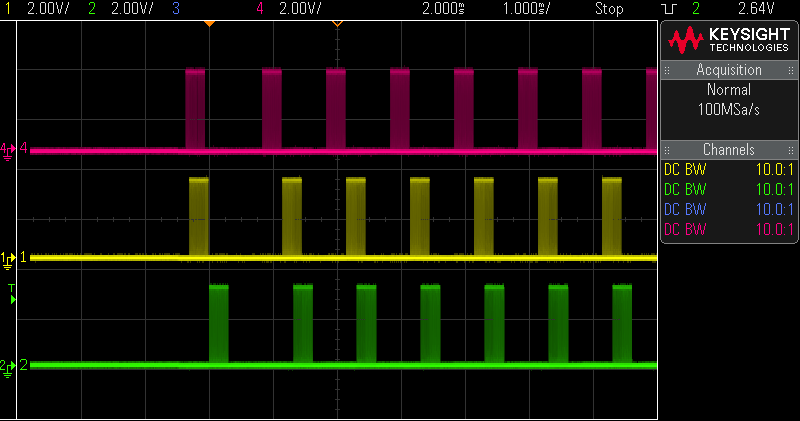
\includegraphics[width=.9\textwidth]{img/scope_9a.png}
	\end{center}
\end{frame}

\begin{frame}{No critical sections}
	\begin{center}
		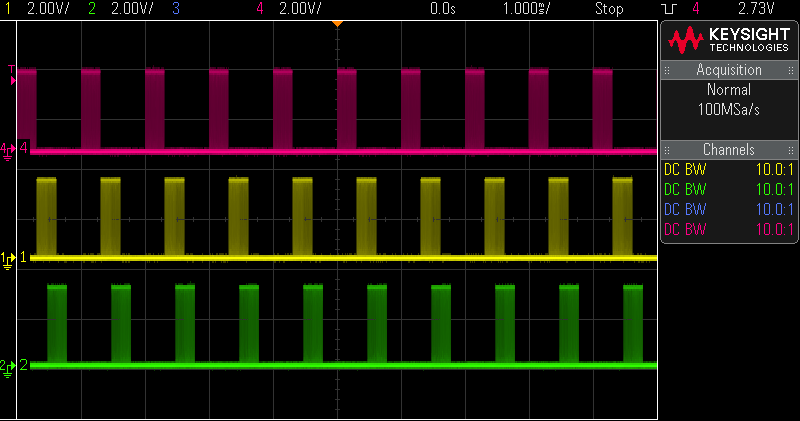
\includegraphics[width=.9\textwidth]{img/scope_9b.png}
	\end{center}
\end{frame}

\begin{frame}{Critical sections}
	\begin{center}
		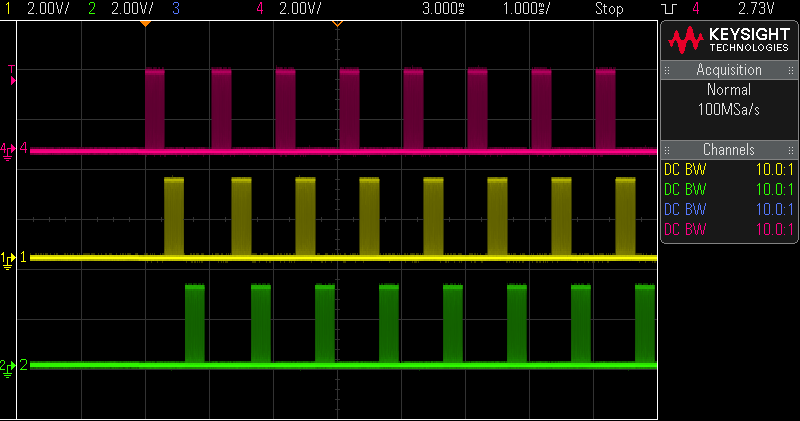
\includegraphics[width=.9\textwidth]{img/scope_9c.png}
	\end{center}
\end{frame}

\begin{frame}{Critical sections}
	\begin{center}
		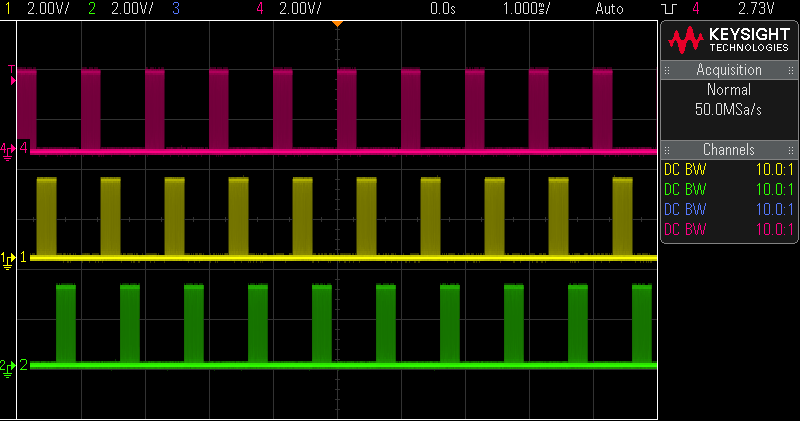
\includegraphics[width=.9\textwidth]{img/scope_9d.png}
	\end{center}
\end{frame}

\subsection[Queues]{Queues}

\begin{frame}{Overview}
	\tableofcontents[currentsection]
\end{frame}

\begin{frame}[fragile]{Queues}
	\begin{itemize}
		\item Producer/consumer layout
		\item More tasks can use the same queue simultaneously
	\end{itemize}
	\begin{center}
		\Cpp
		\begin{lstlisting}
QueueHandle_t myQueue = xQueueCreate(10, sizeof(uint32_t));

xQueueSend(myQueue, (void*) &data, (TickType_t) 0);

xQueueReceive(myQueue, &data, (TickType_t) 0);
		\end{lstlisting}
		\url{https://www.freertos.org/Embedded-RTOS-Queues.html}
	\end{center}
\end{frame}

\begin{frame}{Queues (example)}
	\begin{itemize}
		\item Green task sends every \SI{2}{ms}
		\item Red task listens every \SI{3}{ms}
		\item Yellow task listens every \SI{4}{ms}
	\end{itemize}
\end{frame}

\begin{frame}{Queues (example)}
	\begin{center}
		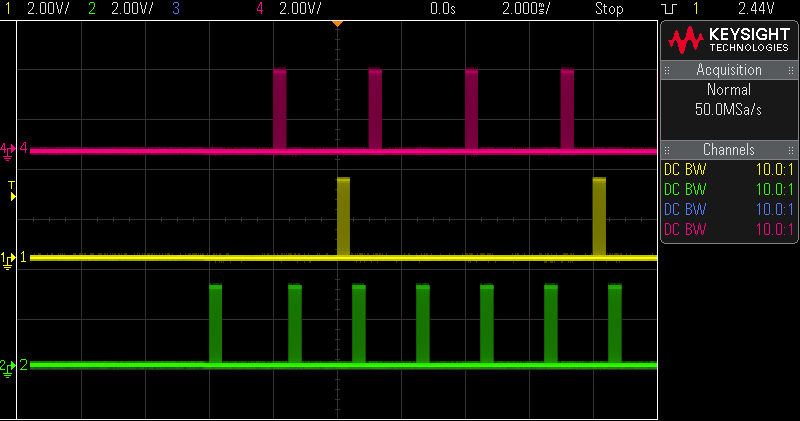
\includegraphics[width=.9\textwidth]{img/scope_10a.png}
	\end{center}
\end{frame}

\begin{frame}{Queues (example)}
	\begin{center}
		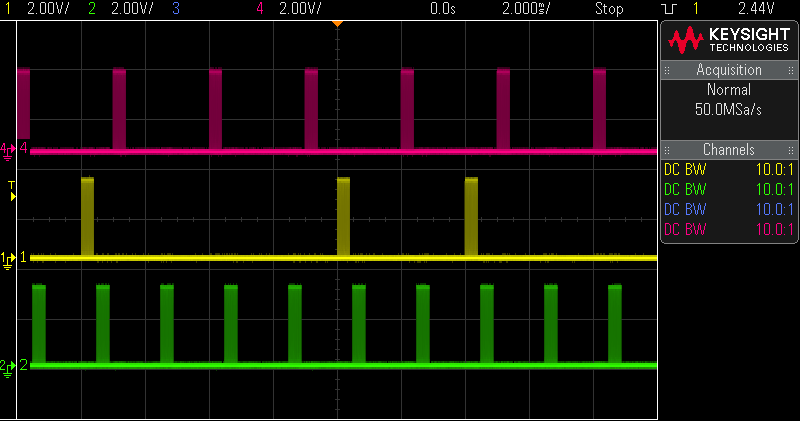
\includegraphics[width=.9\textwidth]{img/scope_10b.png}
	\end{center}
\end{frame}

\begin{frame}{Queues (example)}
	\begin{center}
		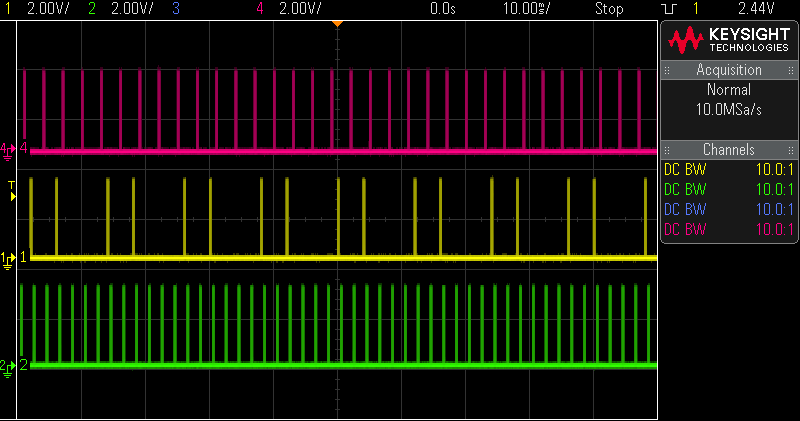
\includegraphics[width=.9\textwidth]{img/scope_10c.png}
	\end{center}
\end{frame}

\begin{frame}
	\begin{center}
		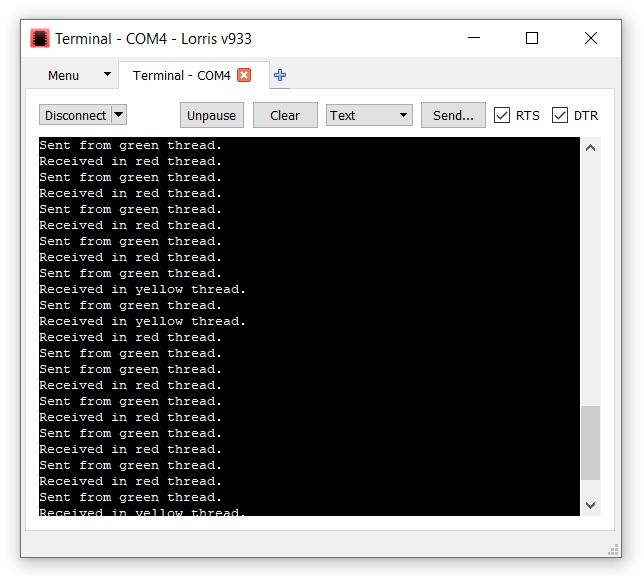
\includegraphics[width=.6\textwidth]{img/queueLorris.png}
	\end{center}
\end{frame}

\begin{frame}{Thank you!}
	\begin{center}
		\includegraphics[height=.6\textheight]{img/scope.jpg}
		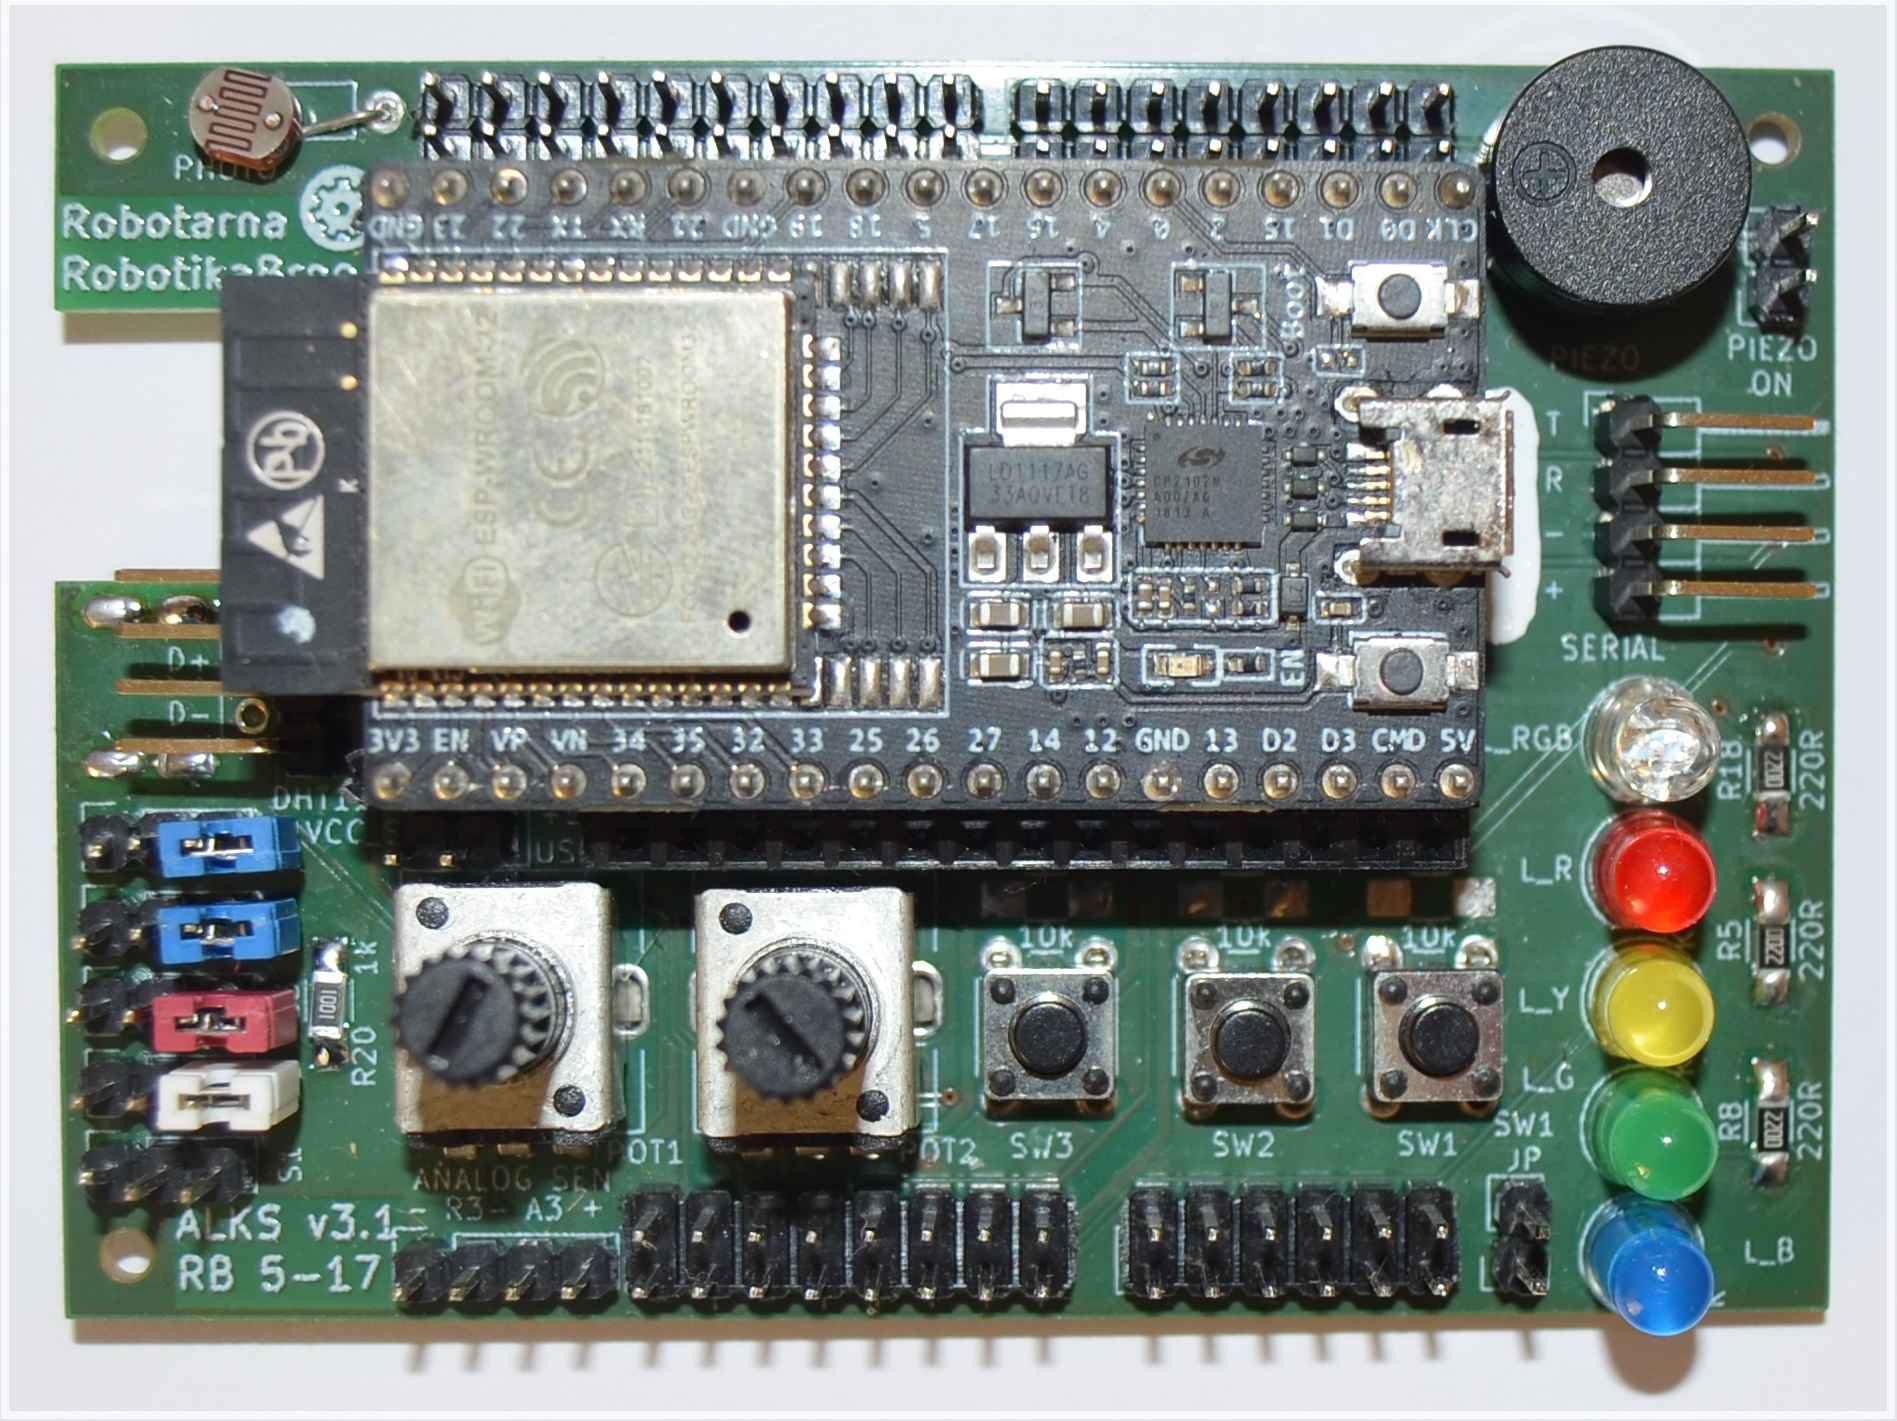
\includegraphics[height=.6\textheight]{img/alks.jpg}
		\vspace{0.5cm}
		\begin{block}{\centering Questions?}
			\centering Bed\v{r}ich Said: 409874@mail.muni.cz
		\end{block}
	\end{center}
\end{frame}

% PlatformIO IDE installation
% https://docs.platformio.org/en/latest/integration/ide/pioide.html

% Espressif32 package for PlatformIO
% https://docs.platformio.org/en/latest/platforms/espressif32.html

% RTOS simulator for Windows
% https://www.freertos.org/FreeRTOS-Windows-Simulator-Emulator-for-Visual-Studio-and-Eclipse-MingW.html

% RTOS simulator for Linux
% https://www.freertos.org/FreeRTOS-simulator-for-Linux.html

\end{document}
